\documentclass[11pt,a4paper]{report}

\usepackage[margin=1in]{geometry}
\usepackage{kotex}
\usepackage{indentfirst}
\usepackage{amsmath,amssymb,amsthm}
\usepackage{booktabs}
\usepackage{longtable}
\usepackage{hyperref}
\usepackage{enumitem}
\usepackage{graphicx}
\usepackage{subcaption}
\graphicspath{{figures/}}
\usepackage{tabularx}
\usepackage{array}

\setlength{\parindent}{1.5em} % 문단 첫 줄 들여쓰기
\setlength{\parskip}{0.3em}   % 문단 사이 간격

\hypersetup{
    colorlinks=true,
    linkcolor=blue,
    citecolor=blue,
    urlcolor=blue
}
\title{The Tempered Fractional Black–Scholes Model as a Diagnostic Pricing Framework: Cross-Asset Evidence Across Option Maturities}
\author{Useong Jeong}
\date{\today}

\begin{document}

\maketitle
\newpage

\chapter*{abstract}
\addcontentsline{toc}{chapter}{abstract}

본 논문은 고전적인 Black--Scholes 모형의 memory-free 구조를 확장하기 위해
Tempered Fractional Black--Scholes, 이하 TFBS, 모형을 도입하고,
이 모형이 실제 옵션 가격 자료에서 Black--Scholes benchmark보다 낮은
validation pricing error를 보일 수 있는지를 분석한다.
Black--Scholes 모형은 옵션 가격결정 이론의 대표적인 기준 모형이지만,
상수 변동성과 Markovian 구조를 가정하기 때문에 옵션 가격에 반영될 수 있는
비국소적 시간 의존성이나 memory effect를 직접적으로 설명하기 어렵다.
이를 보완하기 위해 본 논문은 Black--Scholes PDE의 시간 미분항을
tempered Caputo fractional derivative로 대체한 TFBS 모형을 고려한다.
이때 fractional order $\alpha$는 memory kernel의 형태를,
tempering parameter $\lambda$는 과거 정보의 영향이 시간 lag에 따라
감쇠하는 속도를 조절한다.

실증분석에서는 미국 시장에서 거래되는 주요 주식 및 ETF의 call option chain을
사용하였다. 각 만기별 option chain을 calibration set과 validation set으로 나누고,
calibration set에서 추정한 모형 parameter를 calibration에 사용하지 않은
validation strike에 적용하여 pricing error를 측정하였다.
비교 기준으로는 validation RMSE를 사용하였으며, 옵션 만기를 short, medium,
long maturity bucket으로 구분하여 TFBS 모형의 성능이 특정 만기 구간에서
더 뚜렷하게 나타나는지 분석하였다. 또한 기초자산을 liquid blue-chip equities,
high-attention 또는 event-driven equities, commodity-linked ETFs로 나누어
TFBS의 성능이 자산의 성격에 따라 어떻게 달라지는지 검토하였다.

분석 결과, TFBS 모형은 모든 자산과 모든 만기에서 Black--Scholes benchmark를
일관되게 개선하지는 않았다. 일부 자산에서는 medium 또는 long maturity에서
validation RMSE가 개선되었으나, 다른 자산에서는 개선 효과가 약하거나 오히려
음수로 나타났다. 특히 AMZN은 medium maturity에서 뚜렷한 개선을 보인 반면,
MSFT와 일부 high-attention 자산에서는 TFBS의 추가적인 flexibility가
validation performance 개선으로 이어지지 않았다. 이러한 결과는 TFBS의 성능이
universal하지 않고, maturity-dependent이면서 asset-specific하다는 점을 보여준다.
따라서 본 논문은 TFBS 모형을 Black--Scholes 모형의 보편적 대체재가 아니라,
option surface에 finite-horizon memory-tempering structure가 존재하는지를
확인하기 위한 reduced-form diagnostic pricing model로 해석한다.

\newpage
\tableofcontents

\chapter{Introduction}

\section{Motivation}

Black--Scholes model은 옵션 가격결정 이론에서 가장 기본적인 benchmark model로 사용되어 왔다.
이 model은 기초자산 가격이 기하브라운운동을 따른다는 가정 아래에서 유럽형 옵션 가격을
닫힌 형태로 제시하며, 이후 대부분의 옵션 가격결정 model의 출발점이 되었다 \cite{BlackScholes1973, Merton1973}.
그러나 실제 금융시장에서는 Black--Scholes model의 단순한 가정만으로 설명하기 어려운 현상들이 관찰된다.
대표적으로 implied volatility는 행사가와 만기에 따라 달라지는 volatility smile, skew, term structure를 보이며
\cite{Dupire1994}, asset returns에서는 volatility clustering과 long-range dependence가
중요한 stylized facts로 알려져 있다 \cite{Cont2001}.
또한 rough volatility는 classical Markovian volatility description을 넘어서는 비국소적 시간 구조를 설명하는 framework로 연구되어 왔다 \cite{GatheralJaissonRosenbaum2018}.

이러한 현상들은 옵션 가격이 현재의 기초자산 가격, 행사가, 만기, 이자율, 그리고 일정한 변동성만으로
완전히 설명되기 어렵다는 점을 시사한다.
Black--Scholes framework에서는 현재 기초자산 가격과 고정된 parameter가 주어졌을 때,
과거 가격 경로가 pricing equation에 명시적인 state variable로 등장하지 않는다.
따라서 option surface에 과거 정보의 영향이나 비국소적 시간 의존성이 반영되어 있다면,
이를 설명하기 위해 classical time derivative를 확장하는 접근을 고려할 수 있다.

이러한 memory effect를 수학적으로 반영하는 한 가지 방법은 classical first-order time derivative를
fractional derivative로 대체하는 것이다.
Fractional derivative는 현재 시점의 변화율이 과거 구간의 변화율 전체에 대한 가중 평균에 의존하도록 만들며,
이를 통해 model 안에 time-nonlocal structure를 포함할 수 있다 \cite{Podlubny1999}.
본 연구의 초기 방향은 Black--Scholes PDE의 시간 미분항을 Caputo fractional derivative로 대체한
Fractional Black--Scholes, 이하 FBS, model을 이용하여 옵션 가격의 memory effect를 분석하는 것이었다
\cite{Wyss2000, CarteaDelCastilloNegrete2007}.

그러나 본 연구의 선행실험에서는 기본 FBS model을 실제 option chain에 적용했을 때,
특히 short maturity에서 fractional order 추정이 불안정하고 pricing error가 크게 변동하는 결과가 나타났다.
기본 FBS model의 Caputo memory kernel은 power-law 형태로 감소하므로,
fractional order $\alpha$ 하나가 memory kernel의 형태와 memory effect의 지속성을 동시에 설명해야 한다.
따라서 과거 정보가 option price에 영향을 미치되,
그 영향이 일정한 horizon 안에서 점차 약화될 수 있도록 하는 추가적인 구조가 필요하다.

이에 본 논문은 Tempered Fractional Black--Scholes, 이하 TFBS, model을 중심으로 한다.
TFBS model은 Caputo fractional derivative에 exponential tempering을 도입하여,
fractional memory structure와 memory decay를 분리한다 \cite{SabzikarMeerschaertChen2015}.
이때 fractional order $\alpha$는 memory kernel의 형태를 나타내고,
tempering parameter $\lambda$는 과거 정보의 영향이 time lag에 따라 얼마나 빠르게 감쇠하는지를 조절한다.
따라서 TFBS는 기본 FBS의 untempered power-law memory structure를 보완하면서,
finite-horizon memory effect를 반영할 수 있는 확장된 fractional PDE model로 해석할 수 있다.
\section{Research Question}

본 논문의 핵심 질문은 다음과 같다.

\begin{quote}
Tempered Fractional Black--Scholes model은 classical Black--Scholes model에 비해 옵션 가격의 validation error를 낮출 수 있는가?
\end{quote}

TFBS model은 Black--Scholes model보다 더 많은 파라미터를 포함하므로, calibration data에 대한 in-sample fitting에서는 자연스럽게 더 낮은 오차를 보일 수 있다. 따라서 본 연구는 calibration error가 아니라, calibration에 사용하지 않은 strike에 대한 validation pricing error를 중심으로 model을 비교한다. 각 만기별 option chain을 calibration set과 validation set으로 나눈 뒤, calibration set에서 model 파라미터를 추정하고, validation set에서 예측 성능을 평가한다.

또한 본 논문은 maturity-dependent performance에 초점을 둔다. 옵션을 단기, 중기, 장기 만기 bucket으로 나누고, 각 bucket에서 Black--Scholes model과 TFBS model의 validation RMSE를 비교한다. 본 논문에서 기본적인 만기 구분은 다음과 같다.

\begin{align*}
\text{Short maturity} &:\quad T \leq 30 \text{ days}, \\
\text{Medium maturity} &:\quad 30 < T \leq 180 \text{ days}, \\
\text{Long maturity} &:\quad T > 180 \text{ days}.
\end{align*}

이를 통해 TFBS model의 우위가 전체 만기에서 일괄적으로 나타나는지, 아니면 특정 만기 구간에서만 나타나는지를 분석한다. 마지막으로 본 논문은 asset-dependent performance를 함께 살펴본다. 동일한 TFBS 구조라도 기초자산의 성격에 따라 성능이 달라질 수 있기 때문이다. 본 연구에서는 기초자산을 크게 세 그룹으로 나눈다. 첫째, AAPL, MSFT, GOOGL, AMZN, JPM과 같은 유동성이 높은 우량주이다. 둘째, TSLA, GME, DJT와 같은 high-attention 또는 event-driven 성격의 주식이다. 셋째, GLD, USO와 같은 commodity 또는 spot-linked ETF이다. 이러한 분류를 통해 TFBS의 개선 효과가 단순히 만기 구조에만 의존하는 것이 아니라, 기초자산의 option surface가 얼마나 안정적인 memory-tempering structure를 갖는지에 따라 달라질 수 있음을 확인하고자 한다.

\section{Main Idea}

Black--Scholes model은 본 논문에서 memory-free benchmark로 사용된다~\cite{BlackScholes1973,Merton1973}. 이 model은 현재의 기초자산 가격, 행사가, 만기, 이자율, 변동성에 의해 옵션 가격을 결정하며, 시간 방향으로는 classical first-order derivative를 사용한다. 따라서 Black–Scholes framework에서는 현재 기초자산 가격과 고정된 parameter가 주어졌을 때, 과거 가격 경로가 pricing equation에 명시적인 state variable로 등장하지 않는다.

이러한 한계를 보완하기 위한 자연스러운 첫 번째 확장은 Black--Scholes PDE의 시간 미분항을 Caputo fractional derivative로 대체하는 것이다~\cite{Podlubny1999,Wyss2000}. 이를 Fractional Black--Scholes, 이하 FBS model이라고 부른다. FBS model에서는 fractional order $\alpha$가 memory effect를 반영하는 핵심 parameter로 작용한다. 그러나 기본 FBS model의 Caputo memory kernel은 power-law 형태로 감소하므로, $\alpha$ 하나가 memory kernel의 형태와 memory의 지속성을 동시에 설명해야 한다. 다시 말해, FBS model은 memory effect를 도입하지만 그 memory가 얼마나 빠르게 감쇠하는지를 별도의 parameter로 조절하지 못한다.

본 논문은 이러한 점에서 Tempered Fractional Black--Scholes, 이하 TFBS model을 중심으로 한다. TFBS model은 Caputo fractional derivative에 exponential tempering을 도입하여, memory kernel을 다음과 같은 형태로 해석한다~\cite{SabzikarMeerschaertChen2015}.
\[
K_{\alpha,\lambda}(t)
=
e^{-\lambda t}t^{-\alpha}.
\]

여기서 $\alpha$는 fractional memory kernel의 형태를 나타내고, $\lambda$는 memory effect의 감쇠 속도를 조절한다. 따라서 TFBS model은 memory structure와 memory decay를 분리하여 설명할 수 있다. 특히 $\lambda=0$이면 tempered kernel은 일반 Caputo kernel이 되므로, TFBS는 FBS의 자연스러운 확장이 된다.

본 논문의 주된 실증 분석은 Black--Scholes model과 TFBS model의 validation performance를 비교하는 데 있다. TFBS model은 Black--Scholes model보다 더 많은 parameter를 포함하므로, 단순히 calibration error만 비교하면 추가 parameter로 인한 in-sample fitting 효과를 배제하기 어렵다. 따라서 본 논문은 각 만기별 option chain을 calibration set과 validation set으로 나누고, calibration set에서 추정한 parameter를 validation set의 strike에 적용하여 out-of-sample pricing error를 계산한다. 이때 주요 비교 기준은 validation RMSE이다.

또한 본 논문은 TFBS의 성능이 만기 구조와 기초자산의 성격에 따라 달라질 수 있다는 점에 주목한다. 옵션을 short, medium, long maturity bucket으로 나눈 뒤, 각 bucket에서 TFBS가 Black--Scholes benchmark에 비해 validation RMSE를 얼마나 개선하는지 측정한다. 특히 중기 만기 옵션은 단기 옵션의 microstructure noise와 만기 근처 payoff nonlinearity의 영향이 상대적으로 줄어들면서도, 장기 옵션의 macro 또는 structural uncertainty가 과도하게 지배하지 않는 구간으로 볼 수 있다. 따라서 본 논문은 TFBS의 memory-tempering structure가 중기 만기 옵션에서 더 명확하게 나타날 수 있는지 검토한다.

\section{Contributions}

본 논문의 기여는 크게 세 가지이다.

첫째, 본 논문은 Black--Scholes PDE, FBS PDE, TFBS PDE를 하나의 fractional PDE framework 안에서 정리한다. 특히 Caputo fractional derivative와 tempered Caputo fractional derivative를 도입하고, $\alpha$와 $\lambda$가 각각 memory structure와 memory decay를 담당한다는 해석을 제시한다. 이를 통해 TFBS가 단순히 parameter를 하나 더 추가한 ad hoc model이 아니라, FBS의 untempered memory structure를 보완하는 자연스러운 확장임을 보인다.

둘째, 본 논문은 TFBS PDE의 수치해법과 calibration--validation framework를 구성한다. 시간 방향으로는 L1-type scheme을 이용하여 tempered Caputo derivative를 이산화하고, 공간 방향으로는 finite difference method를 적용한다~\cite{SabzikarMeerschaertChen2015}. 이산화된 문제는 각 time step에서 tridiagonal linear system으로 귀결된다. 이후 옵션 데이터에 대해 만기별로 calibration strike와 validation strike를 분리하고, validation RMSE를 기준으로 Black--Scholes model과 TFBS model을 비교한다. 이는 TFBS가 더 많은 parameter를 갖는다는 점에서 발생할 수 있는 단순 in-sample overfitting 문제를 줄이기 위한 설계이다.

셋째, 본 논문은 TFBS model의 성능이 maturity-dependent이면서 동시에 asset-specific하다는 점을 실증적으로 분석한다. 이를 위해 기초자산을 liquid blue-chip equities, high-attention 또는 event-driven equities, commodity 또는 spot-linked ETFs의 세 그룹으로 나누고, 각 자산에 대해 maturity bucket별 validation pricing error를 비교한다. 이 분석을 통해 TFBS의 개선 효과가 단순히 특정 asset class나 특정 maturity에 의해 자동적으로 결정되는 것이 아니라, 각 option surface의 memory-tempering signature에 따라 달라질 수 있음을 보인다.

\section{Organization of the Thesis}

본 논문의 구성은 다음과 같다. 제2장에서는 classical Black--Scholes model과 그 한계를 정리한다. 제3장에서는 Riemann--Liouville fractional integral, Caputo fractional derivative, tempered Caputo derivative 등 필요한 fractional calculus의 기본 개념을 소개한다. 제4장에서는 FBS model과 TFBS model을 정의하고, FBS의 untempered memory 구조가 갖는 한계를 설명한 뒤, 이를 보완하는 TFBS model을 제시한다.

제5장에서는 TFBS PDE의 finite difference scheme과 calibration--validation 방법론을 제시한다. 특히 L1 scheme을 이용한 tempered Caputo derivative의 이산화, 공간 방향의 finite difference approximation, 그리고 각 time step에서 나타나는 tridiagonal linear system을 설명한다. 제6장에서는 옵션 데이터, asset classification, maturity bucket, parameter grid 등 실험 설계를 설명한다.

제7장에서는 empirical results를 제시한다. Liquid blue-chip equities, high-attention 또는 event-driven equities, commodity 또는 spot-linked ETFs를 구분하고, 각 asset과 maturity bucket에서 TFBS model이 Black--Scholes benchmark에 비해 validation RMSE를 얼마나 개선하는지 비교한다. 제8장에서는 종목별 성능 차이를 설명할 수 있는 candidate drivers를 논의한다. 특히 finite-horizon memory structure, short-maturity noise, option-surface smoothness, event-driven instability, commodity 및 macro factor의 역할을 해석한다. 제9장에서는 grid sensitivity, price source, numerical resolution, maturity bucket 정의, calibration--validation split 등 robustness checks와 model limitations를 정리한다. 마지막으로 제10장에서는 주요 결과를 요약하고, 본 연구의 한계와 향후 연구 방향을 제시한다.

\chapter{Classical Black--Scholes Model and Its Limitations}

\section{The Black--Scholes Framework}

Black--Scholes model은 옵션 가격결정 이론에서 가장 기본적인 benchmark model로 사용된다~\cite{BlackScholes1973,Merton1973}. 이 model의 핵심 가정은 기초자산 가격이 연속시간 확률과정으로 움직이며, 그 dynamics가 기하브라운운동으로 주어진다는 것이다. 기초자산 가격을 $S_t$라 할 때, physical measure 아래에서의 가격과정은 보통 다음과 같이 쓴다.
\[
dS_t = \mu S_t\,dt + \sigma S_t\,dW_t,
\]
여기서 $\mu$는 기초자산의 기대수익률, $\sigma>0$는 상수 변동성, $W_t$는 표준 Brownian motion이다. 또한 무위험자산 $B_t$는
\[
dB_t = rB_t\,dt
\]
를 따른다고 가정한다. 여기서 $r$은 무위험 이자율이다.

옵션 가격결정에서는 physical drift $\mu$ 자체보다 risk-neutral measure 아래에서의 dynamics가 중요하다. 연속 배당수익률을 $q$라고 두면, risk-neutral measure $\mathbb{Q}$ 아래에서 기초자산은 다음을 따른다.
\[
dS_t = (r-q)S_t\,dt + \sigma S_t\,dW_t^{\mathbb{Q}}.
\]
따라서 Black--Scholes model에서 옵션 가격은 기초자산의 현재 가격, 행사가, 만기, 이자율, 배당수익률, 그리고 상수 변동성 $\sigma$에 의해 결정된다. 이때 $\sigma$는 시간과 가격 수준에 의존하지 않는 상수로 가정된다.

본 논문에서는 Black--Scholes model을 이후 fractional model과 비교하기 위한 기준 model로 사용한다. 특히 TFBS model의 성능을 평가할 때, 각 만기별 option chain에 대해 Black--Scholes model의 volatility parameter를 calibration하고, validation strike에서의 pricing error를 비교한다.

\section{Derivation of the Black--Scholes PDE}

기초자산을 underlying asset으로 갖는 유럽형 옵션 가격을 $V(S,t)$라고 하자. $V$가 충분히 smooth하다고 가정하면, It\^o's lemma에 의해
\[
dV
=
\left(
V_t
+
(r-q)S V_S
+
\frac{1}{2}\sigma^2 S^2 V_{SS}
\right)dt
+
\sigma S V_S\,dW_t^{\mathbb{Q}}.
\]
무차익 원리 또는 risk-neutral pricing argument를 적용하면, 옵션 가격은 다음 Black--Scholes PDE를 만족한다~\cite{BlackScholes1973,Merton1973}.
\[
V_t
+
\frac{1}{2}\sigma^2 S^2 V_{SS}
+
(r-q)S V_S
-
rV
=
0.
\]
여기서 $V_t$는 시간 $t$에 대한 미분, $V_S$와 $V_{SS}$는 각각 기초자산 가격 $S$에 대한 1차 및 2차 미분이다.

본 논문에서는 finite difference scheme을 구성할 때 time-to-maturity 변수를 사용하는 것이 편리하므로,
\[
\tau = T-t
\]
를 도입한다. $C(S,\tau)=V(S,T-\tau)$라고 쓰면, $\tau=0$은 만기 시점을 의미하고, $\tau$가 증가할수록 현재 시점에서 만기까지 남은 시간이 길어지는 방향이 된다. 이 변수변환을 적용하면 Black--Scholes PDE는 다음과 같이 쓸 수 있다.
\[
\frac{\partial C}{\partial \tau}
=
\mathcal{L}_{BS} C,
\]
where
\[
\mathcal{L}_{BS} C
=
\frac{1}{2}\sigma^2 S^2 C_{SS}
+
(r-q)S C_S
-
rC.
\]
여기서 $\mathcal{L}_{BS}$는 Black--Scholes spatial operator이다. 이후 FBS 및 TFBS model은 이 식의 왼쪽에 있는 classical first-order time derivative를 fractional 또는 tempered fractional derivative로 대체하는 방식으로 구성된다.

\section{Terminal and Boundary Conditions for Call Options}

유럽형 call option의 payoff는 만기에서
\[
C(S,0) = (S-K)^+
\]
로 주어진다. 여기서 $K$는 행사가이고, $(x)^+=\max(x,0)$이다. 이 조건은 time-to-maturity formulation에서 초기조건 역할을 한다.

공간 방향의 boundary condition은 다음과 같이 설정한다. 먼저 기초자산 가격이 0일 때 call option은 행사될 수 없으므로,
\[
C(0,\tau)=0
\]
로 둔다. 반대로 $S$가 충분히 클 때 call option은 deep in-the-money가 되므로, 옵션 가격은 대략 forward-adjusted intrinsic value에 가까워진다. 따라서 큰 $S_{\max}$에 대해 다음 boundary condition을 사용한다.
\[
C(S_{\max},\tau)
\approx
S_{\max}e^{-q\tau}
-
Ke^{-r\tau}.
\]
수치해법에서는 무한한 공간영역 $S\in[0,\infty)$를 직접 다룰 수 없으므로, 충분히 큰 $S_{\max}$를 정하고 그 구간 $[0,S_{\max}]$ 위에서 finite difference method를 적용한다. 본 논문에서 사용하는 TFBS numerical scheme 역시 같은 terminal condition과 boundary condition을 사용한다.

\section{Closed-Form Black--Scholes Formula}

Black--Scholes PDE는 유럽형 call option에 대해 닫힌 형태의 해를 갖는다~\cite{BlackScholes1973,Merton1973}. 현재 기초자산 가격을 $S_0$, 만기까지의 시간을 $T$, 행사가를 $K$라 하면, continuous dividend yield $q$를 포함한 Black--Scholes call price는
\[
C_{BS}(S_0,K,T,r,q,\sigma)
=
S_0 e^{-qT}N(d_1)
-
K e^{-rT}N(d_2),
\]
where
\[
d_1
=
\frac{
\log(S_0/K)
+
(r-q+\frac{1}{2}\sigma^2)T
}{
\sigma\sqrt{T}
},
\qquad
d_2=d_1-\sigma\sqrt{T}.
\]
여기서 $N(\cdot)$은 표준정규분포의 누적분포함수이다. $q=0$으로 두면 일반적으로 가장 많이 사용되는 non-dividend paying stock에 대한 Black--Scholes formula가 된다.

본 논문에서 Black--Scholes model은 각 만기별로 하나의 volatility parameter $\sigma$를 calibration하는 benchmark로 사용된다. 즉, 만기 $T_j$에 대해 관측된 option prices와 Black--Scholes prices 사이의 squared error를 최소화하는 $\sigma_j$를 선택한다. 이후 같은 만기의 validation strike에서 pricing error를 계산하고, TFBS model의 validation error와 비교한다.

\section{Limitations of the Classical Black--Scholes Model}

Black--Scholes model은 수학적으로 간결하고 옵션 가격결정의 기준점을 제공한다는 점에서 중요하지만, 실제 시장 자료를 설명하는 데에는 몇 가지 한계를 가진다.

\subsection{Constant Volatility Assumption}

Black--Scholes model에서 volatility $\sigma$는 상수로 가정된다. 그러나 실제 옵션시장에서 관측되는 implied volatility는 행사가와 만기에 따라 달라지는 경우가 많다. 즉, 시장에서는 volatility smile, volatility skew, volatility term structure가 나타난다~\cite{Dupire1994,Heston1993}. 이는 하나의 상수 $\sigma$만으로 모든 strike와 maturity의 옵션 가격을 동시에 설명하기 어렵다는 점을 의미한다.

본 논문에서는 각 만기별로 Black--Scholes volatility를 따로 calibration하여 benchmark의 성능을 가능한 한 공정하게 설정한다. 그러나 이 경우에도 같은 만기 안에서 strike별 volatility smile을 완전히 설명하기는 어렵다.

\subsection{Markovian and Memory-Free Structure}

Black--Scholes model의 또 다른 중요한 특징은 Markovian structure이다. 즉, 현재의 기초자산 가격이 주어지면 과거 가격 경로는 미래 dynamics에 직접적으로 영향을 주지 못한다. 그러나 실제 금융시장에서는 long-range dependence와 같이 과거 시장 정보가 현재 가격 형성에 영향을 주는 현상이 관찰되어 왔다~\cite{MandelbrotVanNess1968,ComteRenault1998}. 또한 rough volatility는 long memory와는 구별되지만, classical Markovian volatility description을 넘어서는 관련 비국소적 volatility framework를 제공한다~\cite{GatheralJaissonRosenbaum2018}. 이러한 현상들은 옵션 가격에도 반영될 수 있다. 따라서 memory-free 구조를 갖는 Black--Scholes model만으로는 이러한 비국소적 시간 의존성을 설명하기 어렵다.

\section{Motivation for Fractional Time Dynamics}

위의 한계들은 Black--Scholes model을 확장할 필요성을 제기한다. 특히 시간 방향의 memory effect를 반영하기 위해 classical first-order derivative를 fractional derivative로 대체하는 접근이 자연스럽다. Caputo fractional derivative는 함수의 과거 변화율 전체를 memory kernel을 통해 가중 평균하므로, option price가 과거 정보에 비국소적으로 의존하는 구조를 model에 포함할 수 있다~\cite{Podlubny1999,Caputo1967}.

가장 기본적인 확장은 Black--Scholes PDE의 시간 미분항을 Caputo fractional derivative로 대체하는 FBS model이다~\cite{Wyss2000,Magdziarz2009}. 그러나 기본 FBS model의 memory kernel은 power-law 형태로 감소하며, fractional order $\alpha$ 하나가 memory kernel의 형태와 memory effect의 지속성을 동시에 설명해야 한다. 따라서 memory structure와 memory decay를 분리하여 조절하기 위해서는 추가적인 parameter가 필요하다.

이러한 이유로 본 논문은 exponentially tempered Caputo derivative를 도입한 TFBS model을 중심으로 한다~\cite{SabzikarMeerschaertChen2015}. TFBS model에서는 $\alpha$가 memory kernel의 fractional shape을 나타내고, $\lambda$가 memory effect의 exponential decay를 조절한다. 즉, TFBS는 Black--Scholes model의 memory-free 구조와 FBS model의 untempered long-memory 구조 사이에서, finite-horizon memory를 반영할 수 있는 중간적 확장으로 볼 수 있다.

다음 장에서는 이러한 fractional time dynamics를 엄밀하게 정의하기 위해 Riemann--Liouville fractional integral, Caputo fractional derivative, 그리고 tempered Caputo derivative를 차례로 소개한다.


















\chapter{Fractional Calculus Preliminaries}

\section{Motivation for Fractional Operators}

Classical calculus에서 미분 연산자는 정수 차수로 정의된다. 가령, first-order derivative는 함수의 instantaneous rate of change를 나타내며, Black--Scholes PDE에서도 시간 방향의 변화는 classical first-order derivative로 표현된다. 그러나 이러한 local derivative는 현재 시점 근처의 정보만을 이용하여 변화를 설명한다. 따라서 과거 전체 경로가 현재 상태에 영향을 미치는 memory effect를 직접적으로 표현하기에는 한계가 있다.

Fractional calculus는 미분과 적분의 차수를 정수가 아닌 실수 차수로 확장하는 이론이다~\cite{Podlubny1999}. Fractional derivative는 일반적인 derivative와 달리 non-local operator의 성격을 가진다. 즉, 어떤 시점에서의 fractional derivative는 그 시점의 국소적 변화율뿐 아니라 과거 구간 전체의 함수값 또는 변화율에 의존한다. 이러한 구조 때문에 fractional derivative는 long memory, hereditary effect, anomalous diffusion 등 과거 의존성이 중요한 현상을 수학적으로 모델링하는 데 사용된다.

본 논문에서는 옵션 가격의 시간 방향 dynamics에 memory effect를 포함하기 위해 fractional derivative를 사용한다. 특히 Black--Scholes PDE의 classical time derivative를 Caputo fractional derivative 또는 tempered Caputo fractional derivative로 대체하는 방식을 고려한다. 이 장에서는 이후 FBS 및 TFBS model을 정의하기 위해 필요한 fractional calculus의 기본 개념을 정리한다.

\section{From Repeated Integration to Fractional Integration}

Fractional integral은 정수 차수 반복적분을 실수 차수로 확장한 개념으로 이해할 수 있다. 먼저 함수 $f$가 $[0,T]$에서 적절히 integrable하다고 하자. Classical calculus에서 $f$의 1차 적분은
\[
(I^1 f)(t)
=
\int_0^t f(s)\,ds
\]

로 정의된다. 이를 $n$번 반복한 $n$차 반복적분은 다음 Cauchy formula로 표현된다.
\[
(I^n f)(t)
=
\frac{1}{(n-1)!}
\int_0^t
(t-s)^{n-1}f(s)\,ds,
\qquad n\in\mathbb{N}.
\]

증명은 induction을 통해 얻을 수 있으며, appendix에서 더 자세히 다룰 것이다. 이제 정수 $n$을 양의 실수 $\alpha>0$로 대체하면 Riemann--Liouville fractional integral이 얻어진다~\cite{Podlubny1999}.

\section{Riemann--Liouville and Caputo Fractional Derivatives}

Fractional derivative를 정의하는 가장 고전적인 정의 중 하나는 Riemann--Liouville fractional derivative이다~\cite{Podlubny1999}. 본 논문에서는 $0<\alpha<1$인 $\alpha$만 생각한다.

$0<\alpha<1$에 대해 Riemann--Liouville fractional derivative는
\[
(D_{RL}^{\alpha} f)(t)
=
\frac{d}{dt}
(I^{1-\alpha}f)(t)
=
\frac{d}{dt}
\left[
\frac{1}{\Gamma(1-\alpha)}
\int_0^t
(t-s)^{-\alpha}f(s)\,ds
\right]
\]

로 정의된다. 이 정의는 fractional integral을 먼저 적용한 뒤 classical derivative를 취하는 형태이다.

그러나 option pricing PDE에서는 terminal condition 또는 initial condition을 classical한 형태로 부여하는 것이 중요하다. 이 점에서 Riemann--Liouville derivative보다 Caputo derivative가 더 편리하다. $0<\alpha<1$에 대해 Caputo fractional derivative는 다음과 같이 정의된다~\cite{Caputo1967,Podlubny1999}.
\[
({}^C D_t^\alpha f)(t)
=
(I^{1-\alpha}f')(t)
=
\frac{1}{\Gamma(1-\alpha)}
\int_0^t
(t-s)^{-\alpha}f'(s)\,ds.
\]

즉, Caputo derivative는 먼저 classical derivative $f'(s)$를 취한 뒤, 그 derivative에 대해 fractional integral을 적용한다.

Caputo derivative의 중요한 장점은 상수 함수의 derivative가 0이라는 점이다. 실제로 $f(t)=c$이면 $f'(t)=0$이므로
\[
{}^C D_t^\alpha c = 0.
\]
이는 classical derivative와 같은 성질이며, 초기조건 또는 payoff condition을 다루는 데 자연스럽다. 반면 Riemann--Liouville derivative에서는 상수 함수의 derivative가 일반적으로 0이 아니다. 이러한 이유로 본 논문에서는 option pricing PDE의 시간 미분항을 대체할 때 Caputo derivative를 사용한다.

Caputo derivative는 memory effect를 자연스럽게 포함한다. 위 정의에서 현재 시점 $t$에서의 fractional derivative는 과거 시점 $s\in[0,t]$에서의 변화율 $f'(s)$ 전체에 의존한다. 이때 가중치는
\[
(t-s)^{-\alpha}
\]
로 주어지며, 이는 현재에 가까운 과거일수록 더 큰 weight를 부여하고, 먼 과거일수록 더 작은 weight를 부여한다. 따라서 Caputo derivative는 과거 변화율의 weighted history를 현재 변화율에 반영하는 non-local time derivative로 해석할 수 있다.

\section{Memory Kernel of the Caputo Derivative}

Caputo derivative의 memory structure를 더 명확히 보기 위해 kernel을 따로 쓰면,
\[
K_{\alpha}(t-s)
=
\frac{1}{\Gamma(1-\alpha)}(t-s)^{-\alpha}
\]

이다. 이 kernel은 $0<\alpha<1$일 때 양수이고, time lag $t-s$가 커질수록 감소한다. 즉, 최근의 변화율은 현재 fractional derivative에 더 큰 영향을 주고, 오래된 과거의 변화율은 더 작은 영향을 준다.

그러나 감소 속도는 exponential decay가 아니라 power-law decay이다. Power-law kernel은 오래된 과거에 대해서도 완전히 빠르게 사라지지 않는 tail을 가진다. 이러한 구조는 long memory를 표현하는 데 자연스럽지만, 실제 금융시장에서 과거 정보의 효과가 무한히 지속된다고 보는 것은 지나치게 강한 가정일 수 있다. 특히 옵션 가격에서는 일정 기간의 정보는 중요하게 반영되지만, 매우 오래된 정보의 영향은 시장 상황 변화, 이벤트, macro factor 등에 의해 빠르게 약화될 수 있다.

이 관점에서 기본 Caputo derivative를 사용한 FBS model은 memory effect를 도입하지만, memory의 형태와 지속성을 fractional order $\alpha$ 하나로 동시에 설명해야 한다. 즉, $\alpha$는 memory kernel의 singularity와 decay shape을 모두 조절하지만, memory가 얼마나 빠르게 effective horizon 안에서 사라지는지는 별도의 parameter로 분리되어 있지 않다. 본 논문에서 TFBS model을 도입하는 이유가 여기에 있다.

\section{Tempered Caputo Fractional Derivative}

Tempered fractional derivative는 power-law memory kernel에 exponential damping을 추가하여, memory effect가 시간이 지남에 따라 더 빠르게 감쇠하도록 만든다~\cite{SabzikarMeerschaertChen2015}. 본 논문에서는 다음과 같은 exponentially tempered Caputo-type derivative를 사용한다.
\[
({}^C D_t^{\alpha,\lambda} f)(t)
=
\frac{1}{\Gamma(1-\alpha)}
\int_0^t
e^{-\lambda(t-s)}
(t-s)^{-\alpha}
f'(s)\,ds,
\qquad 0<\alpha<1,\quad \lambda\ge0.
\]
여기서 $\lambda$는 tempering parameter이다. $\lambda=0$이면 exponential factor가 1이 되므로,
\[
{}^C D_t^{\alpha,0}f
=
{}^C D_t^\alpha f.
\]
따라서 tempered Caputo derivative는 ordinary Caputo derivative를 포함하는 확장된 operator이다.

Tempered Caputo derivative의 memory kernel은
\[
K_{\alpha,\lambda}(u)
=
e^{-\lambda u}u^{-\alpha},
\qquad u>0
\]
로 쓸 수 있다. 여기서 $u=t-s$는 time lag이다. 이 kernel은 power-law decay와 exponential decay를 동시에 가진다. 즉, $\alpha$는 fractional memory의 shape을 조절하고, $\lambda$는 먼 과거의 영향을 얼마나 빠르게 감쇠시킬지를 조절한다.

다음 성질은 TFBS model의 parameter interpretation에 중요하다. $0<\alpha<1$ 및 $\lambda\ge0$에 대해
\[
K_{\alpha,\lambda}(u)>0
\]
이고, $u>0$에서 감소한다. 실제로
\[
\log K_{\alpha,\lambda}(u)
=
-\lambda u-\alpha\log u
\]
이므로
\[
\frac{d}{du}\log K_{\alpha,\lambda}(u)
=
-\lambda-\frac{\alpha}{u}<0.
\]
따라서 $K_{\alpha,\lambda}$는 양의 감소 kernel이다. 또한 $\lambda$가 커질수록 exponential damping이 강해져 오래된 과거 정보의 영향은 더 빠르게 줄어든다.

\section{Interpretation of \texorpdfstring{$\alpha$}{alpha} and \texorpdfstring{$\lambda$}{lambda}}

TFBS model에서 fractional order $\alpha$와 tempering parameter $\lambda$는 서로 다른 역할을 한다. 먼저 $\alpha$는 memory kernel의 fractional shape을 결정한다. Caputo-type kernel에서 $\alpha$는 현재 근처의 singularity와 과거 lag에 따른 power-law decay를 조절한다. $\alpha$가 1에 가까워질수록 operator는 classical first-order derivative에 가까운 방향으로 해석될 수 있으며, $\alpha$가 작아질수록 과거 구간 전체에 더 넓게 퍼진 memory contribution을 반영한다.

반면 $\lambda$는 memory effect의 decay rate를 조절한다. $\lambda=0$이면 memory kernel은 pure power-law 형태이고, 이는 FBS model에 해당한다. $\lambda>0$이면 exponential damping이 추가되어 먼 과거의 영향이 더 빠르게 약화된다. 대략적으로 $\lambda$의 역수 $1/\lambda$는 exponential factor $e^{-\lambda u}$가 $e^{-1}$ 수준으로 줄어드는 time scale을 나타내므로, memory effect의 effective horizon을 해석하는 하나의 기준으로 사용할 수 있다. 예를 들어 $\lambda$가 큰 경우, model은 과거 정보의 영향이 존재하더라도 비교적 짧은 horizon 안에서 빠르게 감쇠한다고 해석할 수 있다.

본 논문에서 추정되는 $\alpha$와 $\lambda$는 실제 시장의 memory를 직접 측정한 물리적 parameter라기보다, option surface를 설명하기 위해 calibration된 model-implied parameters이다. 따라서 이 값들은 각 기초자산의 option surface가 보이는 memory-tempering signature로 해석하는 것이 적절하다. 이후 실증분석에서는 각 asset과 maturity bucket에서 추정된 $\alpha$와 $\lambda$가 TFBS의 validation pricing performance와 어떻게 연결되는지 살펴본다.

\section{Connection to the TFBS Model}

본 장에서 정의한 tempered Caputo derivative는 다음 장에서 TFBS PDE를 구성하는 핵심 요소로 사용된다. Classical Black--Scholes PDE는 time-to-maturity variable $\tau$에 대해
\[
\frac{\partial C}{\partial \tau}
=
\mathcal{L}_{BS}C
\]
의 형태를 갖는다. FBS model은 왼쪽의 classical first-order derivative를 Caputo fractional derivative로 대체한 model이고, TFBS model은 이를 다시 tempered Caputo derivative로 확장한 model이다.

즉 TFBS model은 다음과 같은 형태로 정의된다.
\[
{}^C D_\tau^{\alpha,\lambda} C(S,\tau)
=
\mathcal{L}_{BS}C(S,\tau).
\]
여기서 $\mathcal{L}_{BS}$는 Black--Scholes spatial operator이고, ${}^C D_\tau^{\alpha,\lambda}$는 time-to-maturity 방향의 tempered Caputo derivative이다. 이 식은 Black--Scholes model의 memory-free structure와 FBS model의 untempered memory structure를 모두 포함하는 확장된 PDE framework로 볼 수 있다.

다음 장에서는 이 TFBS PDE를 명시적으로 정의하고, terminal condition 및 boundary condition과 함께 option pricing problem으로 정식화한다. 이후 numerical scheme 장에서는 tempered Caputo derivative를 L1 scheme으로 이산화하여 실제 option price를 계산하는 방법을 설명한다.




























\chapter{From FBS to TFBS}

\section{Black--Scholes Operator in Time-to-Maturity Form}

앞 장에서 논의한 fractional time derivative를 option pricing PDE에 적용하기 위해, 먼저 Black--Scholes PDE를 time-to-maturity 변수로 다시 정리한다. 만기까지 남은 시간을
\[
\tau = T-t
\]

라고 두고, 유럽형 call option의 가격을 $C(S,\tau)$라고 쓰자. Classical Black--Scholes PDE는 다음과 같이 표현된다.
\[
\frac{\partial C}{\partial \tau}
=
\mathcal{L}_{BS}C,
\]

where
\[
\mathcal{L}_{BS}C
=
\frac{1}{2}\sigma^2S^2C_{SS}
+
(r-q)SC_S
-
rC.
\]

여기서 $S$는 기초자산 가격, $r$은 무위험 이자율, $q$는 연속 배당수익률, $\sigma$는 volatility parameter이다. Operator $\mathcal{L}_{BS}$는 option price의 공간 방향 변화를 나타내는 Black--Scholes spatial operator이다.

이 formulation에서 Black--Scholes model의 시간 방향 변화는 classical first-order derivative
\[
\frac{\partial C}{\partial \tau}
\]

로 표현된다. 따라서 현재 시점의 변화는 local한 시간 변화율에 의해 결정되며, 과거 경로 전체에 대한 명시적인 memory term은 포함되지 않는다. FBS와 TFBS model은 이 classical time derivative를 fractional derivative 또는 tempered fractional derivative로 대체함으로써 time-nonlocal structure를 도입한다.

\section{Fractional Black--Scholes Model}

가장 자연스러운 첫 번째 확장은 Black--Scholes PDE의 classical first-order time derivative를 Caputo fractional derivative로 대체하는 것이다. 이를 Fractional Black--Scholes, 이하 FBS, model이라고 한다~\cite{Wyss2000,Magdziarz2009}. $0<\alpha<1$에 대해 FBS model은 다음과 같이 쓸 수 있다.
\[
{}^C D_\tau^\alpha C(S,\tau)
=
\mathcal{L}_{BS}C(S,\tau),
\qquad S>0,\quad \tau>0.
\]

여기서 ${}^C D_\tau^\alpha$는 time-to-maturity variable $\tau$에 대한 Caputo fractional derivative이다.

FBS model의 terminal condition은 classical Black--Scholes model과 동일하게 call payoff로 주어진다.
\[
C(S,0)
=
(S-K)^+.
\]

Boundary condition 또한 call option의 기본적인 경제적 성질을 반영하여 다음과 같이 둔다.
\[
C(0,\tau)=0,
\]

and for sufficiently large $S_{\max}$,
\[
C(S_{\max},\tau)
\approx
S_{\max}e^{-q\tau}
-
Ke^{-r\tau}.
\]

FBS model에서 fractional order $\alpha$는 memory effect를 반영하는 핵심 parameter이다. Caputo derivative의 정의에 의해 현재 시점의 fractional derivative는 과거 시점들의 변화율 $C_\tau(S,s)$에 대한 weighted history를 포함한다. 따라서 FBS model은 Black--Scholes model의 memory-free structure를 확장하여, option price의 time dynamics에 non-local memory effect를 반영할 수 있다.

\section{Tempered Fractional Black--Scholes Model}

Tempered Fractional Black--Scholes, 이하 TFBS, model은 FBS model의 Caputo derivative를 tempered Caputo derivative로 대체한 model이다~\cite{SabzikarMeerschaertChen2015}. $0<\alpha<1$ 및 $\lambda\ge0$에 대해, 본 논문에서 사용하는 tempered Caputo-type derivative는 다음과 같은 memory kernel을 갖는다.
\[
K_{\alpha,\lambda}(u)
=
e^{-\lambda u}u^{-\alpha},
\qquad u>0.
\]
이에 따라 TFBS model은 다음과 같이 정의된다.
\[
{}^C D_\tau^{\alpha,\lambda} C(S,\tau)
=
\mathcal{L}_{BS}C(S,\tau),
\qquad S>0,\quad \tau>0.
\]
즉,
\[
{}^C D_\tau^{\alpha,\lambda} C(S,\tau)
=
\frac{1}{\Gamma(1-\alpha)}
\int_0^\tau
e^{-\lambda(\tau-s)}
(\tau-s)^{-\alpha}
\frac{\partial C}{\partial s}(S,s)\,ds.
\]

TFBS model의 terminal condition과 boundary condition은 FBS 및 Black--Scholes model과 동일하게 설정한다.
\[
C(S,0)
=
(S-K)^+,
\]
\[
C(0,\tau)=0,
\]
and
\[
C(S_{\max},\tau)
\approx
S_{\max}e^{-q\tau}
-
Ke^{-r\tau}.
\]

TFBS model에서 $\alpha$와 $\lambda$는 서로 다른 역할을 한다. Fractional order $\alpha$는 memory kernel의 power-law shape을 나타내고, tempering parameter $\lambda$는 memory effect가 시간 lag에 따라 얼마나 빠르게 감쇠하는지를 조절한다. $\lambda$가 커질수록 exponential damping이 강해지므로, 먼 과거의 영향은 더 빠르게 사라진다. 반대로 $\lambda=0$이면 exponential damping이 사라지고, TFBS model은 FBS model로 환원된다.

\section{Relation Between BS, FBS, and TFBS}

TFBS model은 Black--Scholes model과 FBS model을 모두 포함하는 확장된 fractional PDE framework로 이해할 수 있다. 먼저 $\lambda=0$인 경우,
\[
e^{-\lambda u}=1
\]
이므로 tempered memory kernel은 ordinary Caputo memory kernel로 환원된다. 따라서
\[
{}^C D_\tau^{\alpha,0}C
=
{}^C D_\tau^\alpha C.
\]
즉,
\[
\lambda=0
\quad\Longrightarrow\quad
\text{TFBS model reduces to FBS model.}
\]

한편 classical Black--Scholes model은 time derivative가 first-order local derivative로 주어지는 memory-free benchmark이다. 엄밀히 말해 continuous-level에서 tempered Caputo derivative를 단순히 $\alpha=1$로 대입하는 것은 정의역 밖의 limit을 포함하므로 조심해야 한다. 그러나 수치 scheme의 관점에서는 $\alpha$가 1에 가까워질수록 fractional time stepping이 classical first-order time stepping에 가까워지는 방향으로 해석할 수 있다. 따라서 BS, FBS, TFBS는 다음과 같은 관계로 이해할 수 있다.
\[
\text{BS}
\quad\longrightarrow\quad
\text{FBS}
\quad\longrightarrow\quad
\text{TFBS}.
\]
여기서 FBS는 BS의 time derivative에 memory를 도입한 첫 번째 확장이고, TFBS는 FBS의 untempered memory kernel에 exponential decay를 추가한 확장이다.

\section{Interpretation of Model Parameters}

TFBS model에는 세 가지 주요 parameter가 등장한다.
\[
\sigma,\qquad \alpha,\qquad \lambda.
\]
이들은 각각 서로 다른 역할을 갖는다.

먼저 $\sigma$는 Black--Scholes spatial operator에 포함되는 diffusion scale parameter이다. Classical Black--Scholes model에서는 $\sigma$를 volatility로 해석하지만, TFBS model에서는 $\sigma$가 $\alpha$ 및 $\lambda$와 함께 jointly calibrated된다. 따라서 TFBS에서의 $\sigma$는 Black--Scholes implied volatility와 동일하게 해석하기보다, model-specific effective diffusion parameter로 보는 것이 적절하다.

Fractional order $\alpha$는 memory kernel의 shape을 조절한다. $\alpha$는 현재 근처의 singularity와 time lag에 따른 power-law decay를 동시에 결정한다. $\alpha$가 1에 가까울수록 model은 classical time derivative에 가까운 방향으로 움직이고, $\alpha$가 작아질수록 과거 구간 전체에 더 넓게 퍼진 memory contribution을 반영하는 경향이 있다.

Tempering parameter $\lambda$는 memory effect의 decay rate를 조절한다. TFBS memory kernel은
\[
K_{\alpha,\lambda}(u)
=
e^{-\lambda u}u^{-\alpha}
\]
이므로, $\lambda$가 클수록 먼 과거의 weight는 더 빠르게 감소한다. 대략적으로 $\lambda^{-1}$은 exponential factor가 $e^{-1}$ 수준으로 감소하는 time scale로 볼 수 있으므로, memory effect의 effective horizon을 해석하는 하나의 기준으로 사용할 수 있다.

\section{Reduced-Form Interpretation}

본 논문의 TFBS model은 full no-arbitrage stochastic volatility model을 구성하기 위한 목적보다는, option surface에 존재할 수 있는 finite-horizon memory structure를 포착하기 위한 reduced-form fractional PDE model로 사용된다. Fractional Brownian motion이나 long-memory dynamics를 기초자산 가격과정에 직접 도입할 경우, no-arbitrage condition과 관련된 추가적인 수학적 문제가 발생할 수 있다~\cite{Cheridito2003}.

대신 본 연구는 Black--Scholes spatial operator를 유지하면서 time derivative를 tempered fractional derivative로 대체하는 PDE-level extension을 고려한다. 이를 통해 classical Black--Scholes benchmark와 비교 가능한 형태를 유지하면서, option price dynamics에 time-nonlocal memory term을 포함할 수 있다.

따라서 TFBS model은 universal pricing formula라기보다, 특정 option surface가 memory-tempering structure를 보이는지를 분석하기 위한 diagnostic pricing model로 해석된다. 이 관점에서 본 논문의 주된 관심은 TFBS model이 어떤 자산과 어떤 maturity bucket에서 Black--Scholes benchmark보다 낮은 validation pricing error를 보이는지, 그리고 그 결과가 추정된 $\alpha$와 $\lambda$의 structure와 어떻게 연결되는지에 있다.






















\chapter{Numerical Scheme and Calibration Methodology}

\section{Overview}

본 장에서는 TFBS PDE를 수치적으로 풀기 위한 finite difference scheme과, 실제 option data에 model을 calibration하는 방법을 설명한다. TFBS model은 closed-form solution을 일반적으로 갖지 않기 때문에, 각 strike와 maturity에 대해 numerical pricing procedure가 필요하다. 본 논문에서는 time-to-maturity 방향으로는 tempered Caputo derivative에 대한 L1-type discretization을 사용하고, underlying asset price 방향으로는 finite difference method를 적용한다~\cite{SabzikarMeerschaertChen2015}.

이 장의 구성은 다음과 같다. 먼저 TFBS PDE를 time and space grid 위에서 이산화한다. 다음으로 이산화된 scheme이 각 time step에서 tridiagonal linear system으로 귀결됨을 보인다. 이후 Black--Scholes benchmark와 TFBS model의 calibration objective를 정의하고, 마지막으로 validation RMSE와 maturity bucket별 improvement measure를 정의한다.

\section{Time and Space Grids}

TFBS PDE는 time-to-maturity variable $\tau$에 대해 다음과 같이 주어진다.
\[
{}^C D_\tau^{\alpha,\lambda} C(S,\tau)
=
\mathcal{L}_{BS}C(S,\tau),
\]

where
\[
\mathcal{L}_{BS}C
=
\frac{1}{2}\sigma^2S^2C_{SS}
+
(r-q)SC_S
-
rC.
\]

만기까지의 시간을 $T$라고 하자. 시간 구간 $[0,T]$를 $N$개의 subinterval로 나누고,
\[
\Delta \tau = \frac{T}{N},
\qquad
\tau_n = n\Delta \tau,
\qquad n=0,1,\dots,N
\]

라고 둔다. 여기서 $\tau=0$은 option maturity에 해당하며, terminal payoff가 initial condition으로 주어진다.

공간 방향에서는 기초자산 가격 영역 $S\in[0,\infty)$를 직접 다룰 수 없으므로, 충분히 큰 $S_{\max}$를 선택하고 유한 구간 $[0,S_{\max}]$ 위에서 계산한다. 공간 grid는
\[
\Delta S = \frac{S_{\max}}{M},
\qquad
S_j=j\Delta S,
\qquad j=0,1,\dots,M
\]
로 둔다. 수치해 $C_j^n$은
\[
C_j^n \approx C(S_j,\tau_n)
\]

을 의미한다.

Call option의 initial condition과 boundary condition은 다음과 같다.
\[
C_j^0=(S_j-K)^+,
\]
\[
C_0^n=0,
\]

and
\[
C_M^n
\approx
S_{\max}e^{-q\tau_n}
-
Ke^{-r\tau_n}.
\]

따라서 수치 scheme에서 미지수는 interior grid points
\[
j=1,2,\dots,M-1
\]

에서의 option values이다.

\section{L1 Approximation of the Tempered Caputo Derivative}

TFBS model에서 사용하는 tempered Caputo derivative는 다음과 같다.
\[
{}^C D_\tau^{\alpha,\lambda} C(S,\tau)
=
\frac{1}{\Gamma(1-\alpha)}
\int_0^\tau
e^{-\lambda(\tau-s)}
(\tau-s)^{-\alpha}
\frac{\partial C}{\partial s}(S,s)\,ds.
\]

여기서 $0<\alpha<1$이고 $\lambda\ge0$이다.

이 derivative를 시간 grid 위에서 근사하기 위해 L1-type discretization을 사용한다. 먼저 standard Caputo L1 weight를
\[
w_k
=
(k+1)^{1-\alpha}-k^{1-\alpha},
\qquad k=0,1,2,\dots
\]

로 정의한다. Tempering을 반영한 weight는
\[
\widetilde w_k
=
e^{-\lambda k\Delta\tau}w_k
\]

로 둔다. 여기서 $\widetilde w_k$는 exponential tempering factor를 lag grid point $k\Delta\tau$에서 평가한 discrete L1-type tempered weight이다. 따라서 이는 tempered kernel의 exact integral weight라기보다, 본 연구의 computational comparison을 위한 quadrature approximation으로 해석한다. 또한
\[
a_0
=
\frac{1}{(\Delta\tau)^\alpha\Gamma(2-\alpha)}
\]

라고 정의한다.

그러면 $\tau_{n+1}$에서의 tempered Caputo derivative는 다음과 같이 근사된다.
\[
{}^C D_\tau^{\alpha,\lambda} C(S_j,\tau_{n+1})
\approx
a_0
\left[
C_j^{n+1}-C_j^n
+
\sum_{k=1}^{n}
\widetilde w_k
\left(
C_j^{n+1-k}-C_j^{n-k}
\right)
\right].
\]

여기서 첫 번째 항 $C_j^{n+1}-C_j^n$은 가장 최근 time step의 변화량이고, summation term은 과거 time increments의 weighted history이다. $\lambda=0$이면 $\widetilde w_k=w_k$가 되어 ordinary Caputo L1 approximation으로 돌아간다.

이 scheme에서 $\widetilde w_k>0$이며, $\lambda$가 커질수록 먼 과거의 weight가 더 빠르게 감소한다. 이러한 성질은 TFBS model의 memory-decay interpretation과 일치한다. 자세한 weight의 positivity와 decay property는 Appendix에서 다룬다.

\section{Spatial Finite Difference Approximation}

이제 Black--Scholes spatial operator $\mathcal{L}_{BS}$를 공간 grid 위에서 이산화한다. Interior point $S_j$, $j=1,\dots,M-1$에 대해 central difference approximation을 사용한다.
\[
C_S(S_j,\tau_n)
\approx
\frac{C_{j+1}^n-C_{j-1}^n}{2\Delta S},
\]
\[
C_{SS}(S_j,\tau_n)
\approx
\frac{C_{j+1}^n-2C_j^n+C_{j-1}^n}{(\Delta S)^2}.
\]

이를 $\mathcal{L}_{BS}$에 대입하면
\[
(\mathcal{L}_h C^n)_j
=
A_j C_{j-1}^n
+
B_j C_j^n
+
D_j C_{j+1}^n
\]

의 형태가 된다. 여기서
\[
A_j
=
\frac{1}{2}\sigma^2\frac{S_j^2}{(\Delta S)^2}
-
\frac{1}{2}(r-q)\frac{S_j}{\Delta S},
\]
\[
B_j
=
-\sigma^2\frac{S_j^2}{(\Delta S)^2}
-
r,
\]
\[
D_j
=
\frac{1}{2}\sigma^2\frac{S_j^2}{(\Delta S)^2}
+
\frac{1}{2}(r-q)\frac{S_j}{\Delta S}.
\]

따라서 $\mathcal{L}_h$는 interior points 위에서 tridiagonal matrix로 표현된다.

\section{Fully Discrete TFBS Scheme}

TFBS PDE
\[
{}^C D_\tau^{\alpha,\lambda}C
=
\mathcal{L}_{BS}C
\]

에서 time derivative에는 L1 approximation을 적용하고, spatial operator에는 finite difference approximation을 적용한다. 본 논문에서는 spatial operator를 time level $n+1$에서 평가하는 implicit scheme을 사용한다. 따라서 interior point $j=1,\dots,M-1$에 대해
\[
a_0
\left[
C_j^{n+1}-C_j^n
+
\sum_{k=1}^{n}
\widetilde w_k
\left(
C_j^{n+1-k}-C_j^{n-k}
\right)
\right]
=
(\mathcal{L}_h C^{n+1})_j.
\]

이를 정리하면
\[
a_0 C_j^{n+1}
-
(\mathcal{L}_h C^{n+1})_j
=
a_0 C_j^n
-
a_0
\sum_{k=1}^{n}
\widetilde w_k
\left(
C_j^{n+1-k}-C_j^{n-k}
\right).
\]

여기서 오른쪽의 summation term은 이전 time levels에서 이미 계산된 값들만 포함하므로, time step $n+1$에서 known history term으로 취급할 수 있다.

Interior vector를
\[
C_{\mathrm{int}}^n
=
(C_1^n,C_2^n,\dots,C_{M-1}^n)^\top
\]
로 두면, fully discrete scheme은 다음 matrix form으로 쓸 수 있다.
\[
(a_0 I - L_h)C_{\mathrm{int}}^{n+1}
=
a_0 C_{\mathrm{int}}^n
-
a_0 H_{\mathrm{int}}^n
+
b_{\mathrm{bdry}}^{n+1}.
\]
여기서 $L_h$는 Black--Scholes spatial operator의 tridiagonal matrix representation이고,
\[
H_{\mathrm{int}}^n
=
\sum_{k=1}^{n}
\widetilde w_k
\left(
C_{\mathrm{int}}^{n+1-k}
-
C_{\mathrm{int}}^{n-k}
\right)
\]

는 fractional history term이다. 또한 $b_{\mathrm{bdry}}^{n+1}$는 boundary condition에서 오는 correction term이다.

이 식은 각 time step마다 tridiagonal linear system을 푸는 문제로 귀결된다. 따라서 계산량은 일반 dense linear system을 푸는 것보다 훨씬 작으며, Thomas algorithm 또는 banded matrix solver를 이용하여 효율적으로 계산할 수 있다.

\section{Tridiagonal Linear System}

Matrix
\[
A_h=a_0 I-L_h
\]
는 tridiagonal matrix이다. Interior index $j=1,\dots,M-1$에 대해 diagonal과 off-diagonal entries는 다음과 같은 구조를 가진다.
\[
(A_h)_{j,j}=a_0-B_j,
\]
\[
(A_h)_{j,j-1}=-A_j,
\]
\[
(A_h)_{j,j+1}=-D_j.
\]
따라서 time step $n+1$에서 풀어야 하는 system은
\[
A_h C_{\mathrm{int}}^{n+1}
=
R^n
\]
이다. 여기서
\[
R^n
=
a_0 C_{\mathrm{int}}^n
-
a_0 H_{\mathrm{int}}^n
+
b_{\mathrm{bdry}}^{n+1}.
\]

Boundary correction은 특히 마지막 interior point에서 중요하다. $j=M-1$에 대한 spatial operator는 $C_M^{n+1}$을 포함하므로, known boundary value
\[
C_M^{n+1}
=
S_{\max}e^{-q\tau_{n+1}}
-
Ke^{-r\tau_{n+1}}
\]
가 right-hand side에 반영된다. $S=0$ boundary에서는 $C_0^{n+1}=0$이므로 correction이 사라진다.

\section{Interpolation at the Current Underlying Price}

Finite difference scheme은 grid points $S_j$에서 option value를 계산한다. 그러나 실제 market data에서 현재 기초자산 가격 $S_0$가 grid point와 정확히 일치한다고 보장할 수 없다. 따라서 numerical scheme으로 얻은 마지막 time level의 price curve
\[
\{(S_j,C_j^N)\}_{j=0}^{M}
\]
를 이용하여 $S_0$에서의 option price를 interpolation한다.

본 논문에서는 간단한 linear interpolation을 사용한다. 즉, $S_j\le S_0\le S_{j+1}$인 두 grid point를 찾고,
\[
C(S_0,T)
\approx
C_j^N
+
\frac{S_0-S_j}{S_{j+1}-S_j}
\left(
C_{j+1}^N-C_j^N
\right)
\]

으로 계산한다. 이 값이 해당 strike와 maturity에 대한 TFBS model price로 사용된다.

\section{Black--Scholes Benchmark Calibration}

본 논문의 실증 분석에서 Black--Scholes model은 benchmark 역할을 한다. 각 maturity $T_j$에 대해 calibration strike set을 $\mathcal{C}_j$라고 하자. Strike $K_{j,\ell}$에 대한 market price를
\[
P_{j,\ell}^{mkt}
\]
라고 쓴다. Black--Scholes model price는
\[
P_{j,\ell}^{BS}(\sigma)
=
C_{BS}(S_0,K_{j,\ell},T_j,r,q,\sigma)
\]

로 표기한다.

각 maturity에 대해 Black--Scholes volatility는 다음 least-squares problem으로 calibration한다.
\[
\widehat{\sigma}_j^{BS}
=
\arg\min_{\sigma\in\Sigma}
\sum_{\ell\in\mathcal{C}_j}
\left(
P_{j,\ell}^{mkt}
-
P_{j,\ell}^{BS}(\sigma)
\right)^2.
\]
여기서 $\Sigma$는 finite volatility grid이다. 본 논문에서는 closed-form Black--Scholes formula를 사용하여 $P_{j,\ell}^{BS}(\sigma)$를 계산한다.

각 maturity별로 하나의 $\widehat{\sigma}_j^{BS}$를 calibration하는 이유는 maturity-dependent volatility level을 benchmark에 어느 정도 반영하기 위해서이다. 그러나 같은 maturity 안에서 strike별 volatility smile을 완전히 설명하지는 못한다. 이러한 한계가 TFBS model과의 validation comparison에서 중요한 비교 지점이 된다.

\section{TFBS Calibration}

TFBS model은 volatility parameter $\sigma$, fractional order $\alpha$, tempering parameter $\lambda$를 포함한다. 본 논문에서는 $\alpha$를 전체 option surface에 대해 공통으로 선택하고, 각 maturity별로 $\sigma$와 $\lambda$를 calibration한다. 이는 $\alpha$를 asset-level memory shape parameter로 해석하고, $\sigma$와 $\lambda$는 maturity별 price level과 memory decay를 반영하는 parameter로 해석하기 위함이다.

먼저 fixed $\alpha$에 대해, maturity $T_j$의 TFBS parameter는 다음과 같이 calibration한다.
\[
(\widehat{\sigma}_j(\alpha),\widehat{\lambda}_j(\alpha))
=
\arg\min_{\sigma\in\Sigma,\lambda\in\Lambda}
\sum_{\ell\in\mathcal{C}_j}
\left(
P_{j,\ell}^{mkt}
-
P_{j,\ell}^{TFBS}(\alpha,\sigma,\lambda)
\right)^2.
\]

여기서 $\Lambda$는 finite grid for tempering parameter이고,
\[
P_{j,\ell}^{TFBS}(\alpha,\sigma,\lambda)
\]

는 앞에서 설명한 finite difference scheme을 통해 계산된 TFBS option price이다.

이후 $\alpha$는 전체 calibration set에 대한 pooled squared error를 최소화하도록 선택한다.
\[
\widehat{\alpha}
=
\arg\min_{\alpha\in A}
\sum_j
\sum_{\ell\in\mathcal{C}_j}
\left(
P_{j,\ell}^{mkt}
-
P_{j,\ell}^{TFBS}
(\alpha,\widehat{\sigma}_j(\alpha),\widehat{\lambda}_j(\alpha))
\right)^2.
\]

여기서 $A$는 finite grid for fractional order이다.

본 논문에서 calibration은 finite grid search로 수행된다. 따라서 각 objective function은 finite set 위에서 평가되며, 최소값은 항상 존재한다. 실제 계산에서는 먼저 coarse grid를 사용하여 대략적인 최적 parameter region을 찾고, 이후 그 주변에서 local fine grid를 구성하여 parameter를 세분화한다. 이러한 coarse-to-fine approach는 계산량을 줄이면서도 지나치게 거친 grid artifact를 완화하기 위한 방법이다.

\section{Calibration--Validation Split}

TFBS model은 Black--Scholes model보다 더 많은 parameter를 포함하므로, calibration data에 대해서는 자연스럽게 더 낮은 error를 보일 수 있다. 따라서 단순히 in-sample calibration error만 비교하면 TFBS의 실제 pricing performance를 과대평가할 수 있다. 이를 방지하기 위해 본 논문에서는 calibration--validation split을 사용한다.

각 maturity $T_j$에 대해 option strikes를 오름차순으로 정렬한 뒤, 일부 strike는 calibration set $\mathcal{C}_j$에, 나머지 strike는 validation set $\mathcal{V}_j$에 배정한다. 본 논문에서는 기본적으로 alternating split을 사용한다. 즉, 정렬된 strike sequence에서 짝수 index는 calibration set, 홀수 index는 validation set으로 배정한다. 이 방식은 calibration set과 validation set 양쪽에 in-the-money, at-the-money, out-of-the-money strike가 비교적 고르게 포함되도록 하기 위한 것이다.

Calibration set에서 추정된 parameter는 validation set에 그대로 적용된다. 예를 들어 Black--Scholes model의 경우 $\widehat{\sigma}_j^{BS}$를 사용하여 validation strikes의 가격을 계산하고, TFBS model의 경우
\[
(\widehat{\alpha},\widehat{\sigma}_j,\widehat{\lambda}_j)
\]

를 사용하여 validation strikes의 가격을 계산한다. 따라서 validation error는 model이 calibration에 사용하지 않은 strike prices를 얼마나 잘 설명하는지를 측정한다.

\section{Validation RMSE}

Maturity $T_j$의 validation set을 $\mathcal{V}_j$라고 하자. Model $m$의 validation RMSE는 다음과 같이 정의한다.
\[
RMSE_{j}^{val}(m)
=
\sqrt{
\frac{1}{|\mathcal{V}_j|}
\sum_{\ell\in\mathcal{V}_j}
\left(
P_{j,\ell}^{mkt}
-
P_{j,\ell}^{m}
\right)^2
}.
\]

여기서 $m$은 Black--Scholes model 또는 TFBS model을 의미한다.

여러 maturity를 하나의 maturity bucket으로 묶을 때에는 각 expiry의 RMSE를 단순 평균하지 않고, squared error와 observation count를 pooling한다. Bucket $B$에 대해 pooled validation RMSE는
\[
RMSE_{B}^{val}(m)
=
\sqrt{
\frac{
\sum_{j\in B}
\sum_{\ell\in\mathcal{V}_j}
\left(
P_{j,\ell}^{mkt}
-
P_{j,\ell}^{m}
\right)^2
}{
\sum_{j\in B}|\mathcal{V}_j|
}
}.
\]

이 방식은 각 maturity에 포함된 validation option의 개수가 다를 수 있다는 점을 반영한다.

\section{Maturity Buckets and Improvement Measure}

본 논문에서는 maturity-dependent performance를 분석하기 위해 옵션을 세 개의 maturity bucket으로 나눈다. 기본적인 구분은 다음과 같다.
\[
\text{Short maturity}
:
T\le 30\ \text{days},
\]
\[
\text{Medium maturity}
:
30<T\le 180\ \text{days},
\]
\[
\text{Long maturity}
:
T>180\ \text{days}.
\]

각 bucket에서 TFBS model이 Black--Scholes benchmark에 비해 어느 정도 validation error를 줄였는지 측정하기 위해 improvement percentage를 정의한다. Asset $i$와 bucket $B$에 대해
\[
Imp_{i,B}
=
100
\cdot
\frac{
RMSE_{i,B}^{BS}
-
RMSE_{i,B}^{TFBS}
}{
RMSE_{i,B}^{BS}
}.
\]

따라서 $Imp_{i,B}>0$이면 TFBS model이 Black--Scholes model보다 낮은 validation RMSE를 보였다는 뜻이고, $Imp_{i,B}<0$이면 TFBS model이 Black--Scholes benchmark보다 나쁜 validation performance를 보였다는 뜻이다.

이 measure를 통해 본 논문은 TFBS의 성능이 전체 만기에서 일괄적으로 나타나는지, 아니면 medium maturity와 같은 특정 구간에서 더 뚜렷하게 나타나는지를 분석한다. 또한 asset group별로 $Imp_{i,B}$를 비교함으로써 TFBS의 performance가 maturity-dependent일 뿐 아니라 asset-specific한지 살펴본다.

\section{Summary}

본 장에서는 TFBS PDE의 수치해법과 calibration methodology를 제시하였다. Time-to-maturity 방향에서는 tempered Caputo derivative에 대한 L1 approximation을 사용하였고, spatial direction에서는 finite difference method를 적용하였다. 이산화된 TFBS PDE는 각 time step에서 tridiagonal linear system으로 귀결되며, 이를 반복적으로 풀어 option price를 계산한다.

또한 Black--Scholes benchmark와 TFBS model의 calibration objective를 정의하고, calibration--validation split을 통해 out-of-sample pricing error를 평가하는 framework를 구성하였다. 마지막으로 maturity bucket별 validation RMSE와 improvement measure를 정의하였다. 다음 장에서는 이 방법론을 실제 option data에 적용하기 위한 data selection, asset classification, filtering rule, parameter grid design을 설명한다.














\chapter{Data and Experimental Design}

\section{Overview}

본 장에서는 실증분석에 사용한 option data와 numerical experiment의 설계를 설명한다. 앞 장에서는 TFBS PDE를 수치적으로 계산하는 방법과 calibration--validation framework를 정의하였다. 본 장에서는 이를 실제 option chain에 적용하기 위해 어떤 기초자산을 선택하고, 어떤 만기와 strike를 사용하며, market price를 어떻게 정의하는지 설명한다.

본 논문의 실증분석은 세 가지 목적을 갖는다. 첫째, TFBS model이 Black--Scholes benchmark에 비해 validation pricing error를 낮출 수 있는지 확인한다. 둘째, 그 개선이 short, medium, long maturity bucket 중 어느 구간에서 뚜렷하게 나타나는지 분석한다. 셋째, TFBS의 성능이 기초자산의 성격에 따라 어떻게 달라지는지 살펴본다.

이를 위해 본 연구는 option chain data를 수집한 뒤, 각 maturity별로 near-the-money call options를 선택한다. 이후 strike들을 calibration set과 validation set으로 나누고, calibration set에서 추정된 parameters를 validation set의 option prices에 적용하여 out-of-sample pricing performance를 평가한다.

\section{Option Data}

본 연구에서는 미국 시장에서 거래되는 equity options 및 ETF options를 대상으로 한다. 각 기초자산에 대해 현재 기초자산 가격 $S_0$와 option chain data를 수집하고, call option만을 분석 대상으로 사용한다. Put option은 본 연구의 범위에서 제외한다. 이는 call option에 대해 Black--Scholes formula와 boundary condition을 일관되게 설정하고, TFBS numerical scheme과 benchmark comparison을 단순화하기 위함이다. 다만 본 연구의 PDE formulation과 Black--Scholes benchmark는 European-style call pricing framework에 기반한다. 미국 시장의 equity options와 ETF options는 일반적으로 American-style exercise feature를 가질 수 있으므로, 본 연구의 empirical results는 absolute pricing accuracy가 아니라 동일한 European-style approximation 아래에서의 relative validation comparison으로 해석한다.

각 option contract는 다음 정보를 포함한다.
\[
\text{expiry},\quad T,\quad K,\quad P^{mkt},\quad \text{bid},\quad \text{ask},\quad \text{lastPrice},
\]
where $T$ is the time to maturity, $K$ is the strike price, and $P^{mkt}$ is the market price proxy used in calibration and validation.

만기까지의 시간은 calendar day 기준으로 계산한 뒤 year fraction으로 변환한다. 즉, 만기까지 남은 날짜 수를 $DTE$라고 하면,
\[
T = \frac{DTE}{365.25}
\]
로 둔다.

\section{Market Price Proxy}

이상적으로는 option market price로 bid--ask midpoint를 사용하는 것이 바람직하다. Bid price와 ask price가 모두 양수이고, ask price가 bid price 이상일 때 midpoint는
\[
P^{mid}
=
\frac{\text{bid}+\text{ask}}{2}
\]
로 정의된다. 또한 bid--ask spread가 지나치게 큰 option은 market microstructure noise가 크다고 볼 수 있으므로, 실험 설계상 제외하는 것이 자연스럽다.

본 논문에서는 market price proxy를 다음과 같이 해석한다.
\[
P^{mkt}_{j,\ell}
=
\begin{cases}
P^{mid}_{j,\ell}, & \text{if reliable bid--ask midpoint is available},\\
P^{last}_{j,\ell}, & \text{otherwise}.
\end{cases}
\]
여기서 $j$는 maturity index, $\ell$은 strike index를 나타낸다. 실제 실험에서는 public data의 제약으로 인해 lastPrice가 사용되는 경우가 많으며, 이는 short maturity options에서 특히 noise를 유발할 수 있다.

\section{Filtering Rules and Maturity Selection}

Option chain에는 deep in-the-money 또는 deep out-of-the-money options, bid--ask spread가 큰 options, 거래가 거의 없는 options 등이 포함될 수 있다. 이러한 contracts는 calibration 결과를 불안정하게 만들 수 있으므로, 본 연구에서는 near-the-money call options를 중심으로 분석한다.

먼저 moneyness를
\[
m = \frac{K}{S_0}
\]
로 정의한다. 여기서 $K$는 strike price이고, $S_0$는 현재 기초자산 가격이다. 본 연구에서는 기본적으로 다음 범위에 있는 options를 후보로 사용한다.
\[
m_{\min} \leq \frac{K}{S_0} \leq m_{\max}.
\]
실험에서는 $m_{\min}=0.70$, $m_{\max}=1.30$과 같은 넓은 범위를 먼저 설정한 뒤, 각 maturity에서 $m=1$에 가까운 strike들을 선택한다. 즉, at-the-money 근처의 options를 우선적으로 사용한다.

만기 선택에서도 균형이 필요하다. 단순히 가장 가까운 expiry부터 선택하면 short maturity options에 표본이 과도하게 몰릴 수 있다. 본 연구는 short, medium, long maturity bucket을 모두 포함하기 위해 target DTE 방식을 사용한다. 예를 들어 다음과 같은 target days to expiration을 설정한다.
\[
14,\ 30,\ 60,\ 90,\ 120,\ 150,\ 180,\ 210,\ 270,\ 360.
\]
각 target DTE에 대해 실제 option chain에서 가장 가까운 expiry를 선택한다. 이 방식은 maturity distribution이 한쪽으로 치우치는 것을 방지하고, maturity-dependent performance를 분석하기 위한 표본을 확보하는 데 목적이 있다.

각 maturity에서는 현재 기초자산 가격에 가장 가까운 strike들을 선택한다. 구체적으로 $|K/S_0-1|$이 작은 순서대로 일정 개수의 call options를 선택한다. 본 연구의 기본 numerical experiments에서는 각 maturity별로 8개의 strike를 선택한다. 이후 이 strike들은 calibration set과 validation set으로 나뉜다.

\section{Maturity Buckets}

본 논문은 TFBS의 성능이 maturity에 따라 달라질 수 있다는 점에 초점을 둔다. 이를 위해 각 option을 maturity에 따라 세 개의 bucket으로 나눈다.
\[
\text{Short maturity}
:
T\le 30\ \text{days},
\]
\[
\text{Medium maturity}
:
30<T\le 180\ \text{days},
\]
\[
\text{Long maturity}
:
T>180\ \text{days}.
\]

Short maturity options는 만기 근처 payoff의 비선형성, 높은 gamma sensitivity, stale lastPrice, bid--ask noise 등 market microstructure effects에 크게 영향을 받을 수 있다. 반면 long maturity options는 interest rate, dividend expectation, macro factor, structural uncertainty의 영향을 더 크게 받을 수 있다. Medium maturity options는 이 두 효과가 상대적으로 덜 극단적인 구간으로 볼 수 있으며, 본 논문은 이 구간에서 memory-tempering structure가 더 명확하게 나타날 가능성에 주목한다.

다만 이 bucket definition은 절대적인 기준이라기보다 empirical classification이다. 따라서 robustness check에서는 medium maturity의 기준을 다소 조정하여 결과가 유지되는지 확인할 수 있다.

\section{Asset Classification}

TFBS의 성능은 maturity뿐 아니라 기초자산의 성격에 따라 달라질 수 있다. 본 연구에서는 기초자산을 다음 세 그룹으로 분류한다.

\begin{table}[htbp]
\centering
\small
\begin{tabularx}{\textwidth}{
@{}
>{\raggedright\arraybackslash}p{0.28\textwidth}
>{\raggedright\arraybackslash}p{0.31\textwidth}
>{\raggedright\arraybackslash}X
@{}
}
\toprule
Asset class & Tickers & Interpretation \\
\midrule
Liquid blue-chip equities
& AAPL, MSFT, GOOGL, AMZN, JPM
& 유동성이 높은 대형주 \\
\midrule
High-attention / event-driven equities
& TSLA, GME, DJT
& 관심도, 이벤트, 투기적 수요의 영향이 큰 주식 \\
\midrule
Commodity / spot-linked ETFs
& GLD, USO
& 금, 원유 등 commodity factor와 연결된 ETF \\
\bottomrule
\end{tabularx}
\caption{Asset classification used in the empirical analysis.}
\label{tab:asset_classification}
\end{table}

첫 번째 그룹은 liquid blue-chip equities이다. 이 그룹은 option chain이 비교적 풍부하고, 시장 유동성이 높은 대형주로 구성된다. AAPL, MSFT, GOOGL, AMZN, JPM이 여기에 포함된다. 이 그룹은 TFBS가 안정적인 option surface에서 어떻게 작동하는지를 확인하기 위한 기준군으로 사용된다.

두 번째 그룹은 high-attention 또는 event-driven equities이다. TSLA, GME, DJT가 이 그룹에 포함된다. 이 자산들은 retail attention, event risk, speculative demand, jump-like movement의 영향을 강하게 받을 수 있다. 따라서 TFBS가 이들 자산에서 안정적인 memory structure를 포착하는지, 아니면 parameter instability를 보이는지 확인할 수 있다.

세 번째 그룹은 commodity 또는 spot-linked ETFs이다. GLD와 USO는 각각 금과 원유 관련 시장 요인을 반영하는 ETF로 볼 수 있다. 이러한 자산은 개별 기업의 earnings나 firm-specific news보다 macro factor, commodity cycle, futures market structure의 영향을 더 크게 받을 수 있다. 따라서 TFBS의 performance가 equity options와 다른 maturity pattern을 보일 수 있다.

\section{Parameter Grid Design}

본 연구에서는 calibration을 finite grid search로 수행한다. TFBS model은 closed-form formula를 갖지 않으므로, 각 parameter combination에 대해 numerical PDE solver를 사용하여 option price를 계산한다. 따라서 parameter grid를 지나치게 촘촘하게 설정하면 계산량이 크게 증가한다. 반대로 grid가 너무 거칠면 parameter estimates가 grid artifact에 의해 왜곡될 수 있다.

이를 완화하기 위해 본 연구는 coarse-to-fine grid strategy를 사용한다. 먼저 coarse grid에서 전체적인 parameter region을 탐색한 뒤, 각 maturity별 coarse optimum 주변에서 local fine grid를 구성한다. 이 방식은 계산량을 줄이면서도 parameter estimates가 지나치게 거친 grid에 의해 결정되는 문제를 완화한다.

TFBS calibration에 사용되는 parameter sets는 다음과 같이 표현된다.
\[
A=\{\alpha_1,\dots,\alpha_{N_\alpha}\},
\]
\[
\Sigma=\{\sigma_1,\dots,\sigma_{N_\sigma}\},
\]
\[
\Lambda=\{\lambda_1,\dots,\lambda_{N_\lambda}\}.
\]
여기서 $A$는 fractional order grid, $\Sigma$는 volatility grid, $\Lambda$는 tempering parameter grid이다.

본 연구에서는 asset group에 따라 grid range를 조정한다. 예를 들어 blue-chip equities에서는 volatility range가 상대적으로 낮게 설정될 수 있는 반면, high-attention 또는 event-driven equities에서는 높은 implied volatility를 반영하기 위해 더 넓은 $\sigma$ grid가 필요하다. 마찬가지로 $\lambda$ grid도 일부 자산에서 높은 tempering value가 선택될 수 있으므로, boundary effect를 줄이기 위해 충분히 넓게 설정한다.

\section{Calibration--Validation Design}

각 maturity $T_j$에 대해 선택된 strike set을 오름차순으로 정렬한다. 본 연구에서는 calibration과 validation을 분리하기 위해 alternating split을 사용한다. 즉, 정렬된 strike sequence에서 짝수 index에 해당하는 strike는 calibration set에, 홀수 index에 해당하는 strike는 validation set에 배정한다. 이를 수식으로 쓰면,
\[
\mathcal{C}_j
=
\{K_{j,\ell}:\ell\ \text{is even}\},
\]
\[
\mathcal{V}_j
=
\{K_{j,\ell}:\ell\ \text{is odd}\}.
\]

이 방식은 calibration set과 validation set이 모두 in-the-money, at-the-money, out-of-the-money 영역을 포함하도록 하기 위한 것이다. Random split을 사용할 수도 있지만, option prices는 strike에 따라 구조적인 변화를 보이므로, strike 순서를 고려한 alternating split이 보다 안정적인 비교를 제공한다.

Calibration set $\mathcal{C}_j$에서 Black--Scholes volatility와 TFBS parameters를 추정한 뒤, 같은 maturity의 validation set $\mathcal{V}_j$에 대해 pricing error를 계산한다. 따라서 validation RMSE는 model이 calibration에 사용하지 않은 strike prices를 얼마나 잘 설명하는지를 측정한다.

\section{Empirical Questions}

본 연구의 empirical analysis는 다음 세 가지 질문을 중심으로 진행된다.

첫째, TFBS model은 Black--Scholes benchmark에 비해 validation pricing error를 낮추는가? 이를 확인하기 위해 각 asset과 maturity bucket에서 Black--Scholes model과 TFBS model의 validation RMSE를 비교한다.

둘째, TFBS의 improvement는 medium maturity bucket에서 더 뚜렷하게 나타나는가? 본 논문은 short, medium, long maturity bucket을 구분하고, 각 bucket별 improvement percentage
\[
Imp_{i,B}
=
100
\cdot
\frac{
RMSE_{i,B}^{BS}
-
RMSE_{i,B}^{TFBS}
}{
RMSE_{i,B}^{BS}
}
\]
를 계산한다. 이를 통해 TFBS의 우위가 특정 maturity bucket에 집중되는지 분석한다.

셋째, TFBS의 performance는 asset class에 따라 어떻게 달라지는가? 같은 blue-chip group 안에서도 AAPL, MSFT, GOOGL, AMZN, JPM의 option surface는 서로 다른 memory-tempering signature를 가질 수 있다. 또한 high-attention equities와 commodity-linked ETFs에서는 event risk, speculative demand, macro factor, commodity cycle이 option price에 영향을 줄 수 있다. 따라서 본 연구는 TFBS의 성능을 universal model performance가 아니라 maturity-dependent and asset-specific performance로 해석한다.















\chapter{Empirical Results Across Assets}

\section{Overview of Validation Results}

본 장에서는 제6장에서 설명한 calibration--validation framework를 여러 기초자산의 option chain에 적용한 결과를 제시한다. 본 논문의 목적은 특정 하나의 자산에서 TFBS model이 잘 작동한다는 것을 보이는 것이 아니라, TFBS의 validation performance가 maturity bucket과 asset class에 따라 어떻게 달라지는지를 분석하는 데 있다. 따라서 본 장에서는 liquid blue-chip equities, high-attention 또는 event-driven equities, commodity 또는 spot-linked ETFs를 차례로 살펴보고, 각 asset과 maturity bucket에서 TFBS가 Black--Scholes benchmark에 비해 validation RMSE를 얼마나 개선하는지 비교한다.

본 장의 핵심 성능 지표는 improvement percentage이다. Asset $i$와 maturity bucket $B$에 대해 improvement를
\[
Imp_{i,B}
=
100
\cdot
\frac{
RMSE_{i,B}^{BS}
-
RMSE_{i,B}^{TFBS}
}{
RMSE_{i,B}^{BS}
}
\]
로 정의한다. 따라서 $Imp_{i,B}>0$이면 TFBS model이 Black--Scholes benchmark보다 낮은 validation RMSE를 보였다는 뜻이고, $Imp_{i,B}<0$이면 TFBS model이 더 높은 validation RMSE를 보였다는 뜻이다.

Figure~\ref{fig:cross_asset_improvement_heatmap}은 전체 asset universe에 대한 maturity-bucket별 improvement를 heatmap으로 나타낸 것이다. 전체적으로 볼 때, TFBS model은 모든 asset과 모든 maturity bucket에서 Black--Scholes benchmark를 일괄적으로 개선하지 않는다. 일부 자산에서는 medium 또는 long maturity에서 개선이 나타나지만, 다른 자산에서는 improvement가 약하거나 음수로 나타난다. 이는 TFBS model의 성능이 universal하지 않고, maturity-dependent이면서 asset-specific하다는 본 논문의 핵심 관점과 일치한다.

\begin{figure}[htbp]
\centering
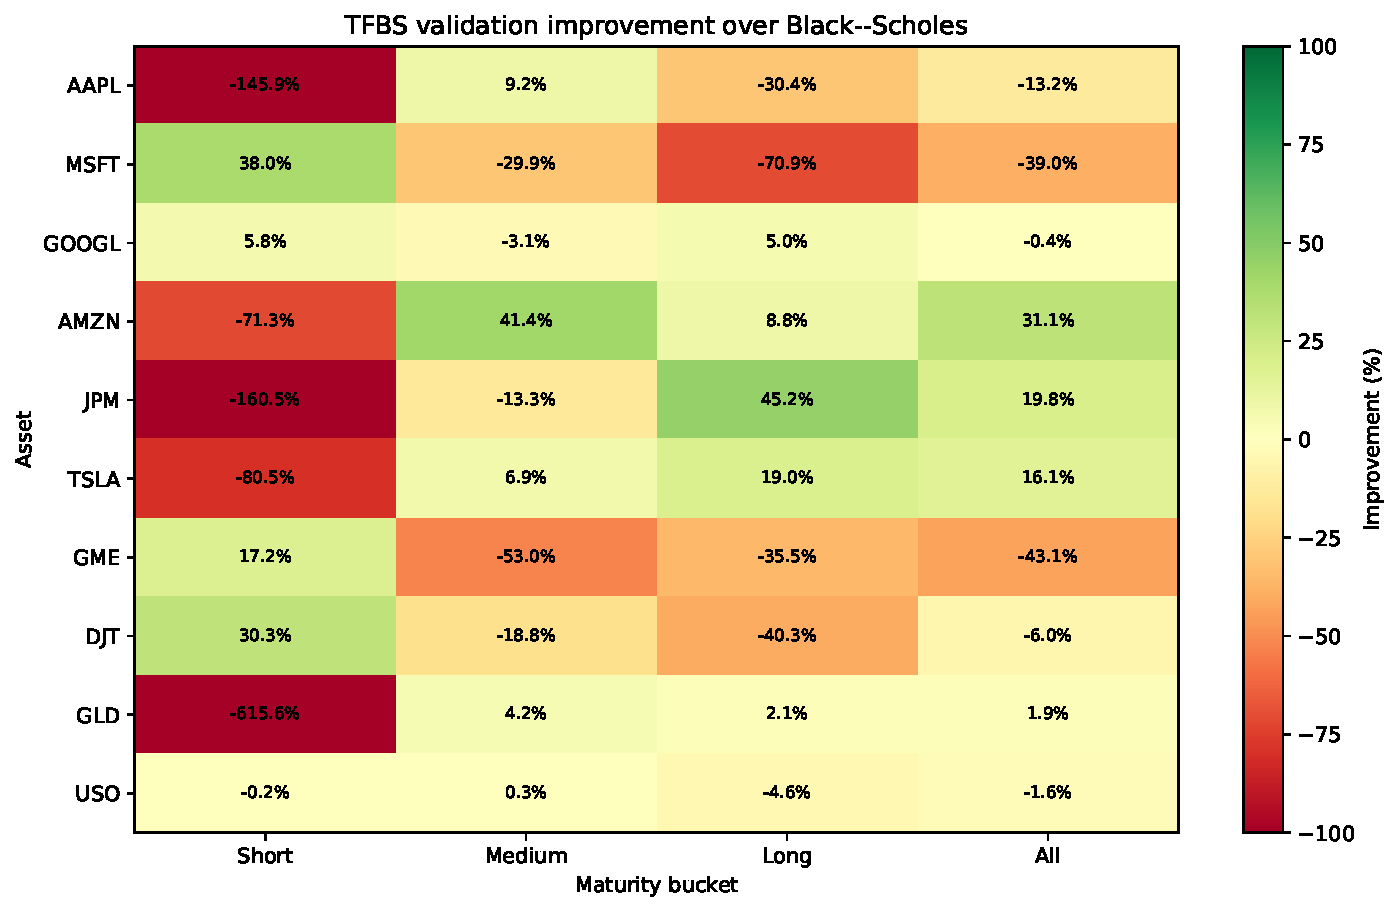
\includegraphics[width=0.92\textwidth]{fig7_1_cross_asset_improvement_heatmap.pdf}
\caption{Validation RMSE improvement of TFBS relative to Black--Scholes across assets and maturity buckets. The color scale is clipped at $\pm100\%$ for readability.}
\label{fig:cross_asset_improvement_heatmap}
\end{figure}

Table~\ref{tab:cross_asset_summary}는 각 asset과 maturity bucket에 대한 validation RMSE와 improvement를 정리한 것이다. Short bucket의 경우 많은 asset에서 expiry 수가 하나뿐이므로, short-maturity result는 표본 수가 작고 market microstructure noise에 민감하다는 점을 고려해야 한다. 따라서 본 장의 주요 해석은 medium, long, 그리고 all-bucket 결과를 중심으로 한다.

\begin{table}[htbp]
\centering
\scriptsize
\begin{tabular}{llrrrr}
\toprule
Asset & Bucket & $n_{\mathrm{exp}}$ & $RMSE^{BS}$ & $RMSE^{TFBS}$ & Improvement \\
\midrule
AAPL & Short  & 1 & 0.2667 & 0.6560 & $-145.9\%$ \\
AAPL & Medium & 5 & 0.6775 & 0.6150 & $9.2\%$ \\
AAPL & Long   & 3 & 0.7515 & 0.9803 & $-30.4\%$ \\
AAPL & All    & 9 & 0.6717 & 0.7604 & $-13.2\%$ \\
\midrule
MSFT & Short  & 1 & 0.4964 & 0.3078 & $38.0\%$ \\
MSFT & Medium & 5 & 0.4849 & 0.6298 & $-29.9\%$ \\
MSFT & Long   & 3 & 0.4740 & 0.8101 & $-70.9\%$ \\
MSFT & All    & 9 & 0.4826 & 0.6706 & $-39.0\%$ \\
\midrule
GOOGL & Short  & 1 & 1.3858 & 1.3053 & $5.8\%$ \\
GOOGL & Medium & 5 & 1.7936 & 1.8497 & $-3.1\%$ \\
GOOGL & Long   & 3 & 1.4600 & 1.3872 & $5.0\%$ \\
GOOGL & All    & 9 & 1.6466 & 1.6527 & $-0.4\%$ \\
\midrule
AMZN & Short  & 1 & 0.1251 & 0.2142 & $-71.3\%$ \\
AMZN & Medium & 5 & 0.5105 & 0.2991 & $41.4\%$ \\
AMZN & Long   & 3 & 0.3523 & 0.3213 & $8.8\%$ \\
AMZN & All    & 9 & 0.4334 & 0.2987 & $31.1\%$ \\
\midrule
JPM & Short  & 1 & 0.2227 & 0.5800 & $-160.5\%$ \\
JPM & Medium & 5 & 0.7195 & 0.8153 & $-13.3\%$ \\
JPM & Long   & 3 & 1.3800 & 0.7566 & $45.2\%$ \\
JPM & All    & 9 & 0.9633 & 0.7730 & $19.8\%$ \\
\midrule
TSLA & Short  & 1 & 0.1743 & 0.3145 & $-80.5\%$ \\
TSLA & Medium & 5 & 0.7447 & 0.6935 & $6.9\%$ \\
TSLA & Long   & 3 & 1.9223 & 1.5575 & $19.0\%$ \\
TSLA & All    & 9 & 1.2422 & 1.0425 & $16.1\%$ \\
\midrule
GME & Short  & 1 & 0.0661 & 0.0547 & $17.2\%$ \\
GME & Medium & 4 & 0.1256 & 0.1921 & $-53.0\%$ \\
GME & Long   & 3 & 0.1535 & 0.2080 & $-35.5\%$ \\
GME & All    & 8 & 0.1298 & 0.1857 & $-43.1\%$ \\
\midrule
DJT & Short  & 1 & 0.3182 & 0.2218 & $30.3\%$ \\
DJT & Medium & 5 & 0.2481 & 0.2948 & $-18.8\%$ \\
DJT & Long   & 2 & 0.1542 & 0.2163 & $-40.3\%$ \\
DJT & All    & 8 & 0.2490 & 0.2639 & $-6.0\%$ \\
\midrule
GLD & Short  & 1 & 0.1168 & 0.8360 & $-615.6\%$ \\
GLD & Medium & 5 & 1.0695 & 1.0242 & $4.2\%$ \\
GLD & Long   & 4 & 5.9478 & 5.8233 & $2.1\%$ \\
GLD & All    & 10 & 3.8372 & 3.7628 & $1.9\%$ \\
\midrule
USO & Short  & 1 & 2.7622 & 2.7664 & $-0.2\%$ \\
USO & Medium & 4 & 3.3815 & 3.3699 & $0.3\%$ \\
USO & Long   & 3 & 3.2305 & 3.3800 & $-4.6\%$ \\
USO & All    & 8 & 3.2534 & 3.3044 & $-1.6\%$ \\
\bottomrule
\end{tabular}
\caption{Cross-asset validation performance of BS and TFBS by maturity bucket.}
\label{tab:cross_asset_summary}
\end{table}

\section{Blue-Chip Equities}

먼저 liquid blue-chip equities group을 살펴본다. 이 그룹에는 AAPL, MSFT, GOOGL, AMZN, JPM이 포함된다. 이들은 비교적 유동성이 높은 대형주이지만, 결과는 상당히 이질적으로 나타난다. 즉, blue-chip 여부 자체가 TFBS의 성능을 결정하지 않는다.

AMZN은 blue-chip group에서 가장 명확한 positive case이다. Medium bucket에서 TFBS는 Black--Scholes 대비 약 $41.4\%$의 validation RMSE reduction을 보였고, Long bucket에서도 약 $8.8\%$의 improvement를 보였다. All bucket 기준으로도 improvement는 약 $31.1\%$이다. 이는 AMZN option surface에서 TFBS의 memory-tempering structure가 validation strike로 비교적 잘 일반화되었음을 시사한다.

반면 MSFT는 명확한 negative case로 나타난다. Short bucket에서는 positive improvement가 관찰되지만, 표본이 하나의 expiry에 불과하므로 강하게 해석하기 어렵다. Medium bucket에서는 $-29.9\%$, Long bucket에서는 $-70.9\%$의 negative improvement가 나타났고, All bucket에서도 $-39.0\%$로 TFBS가 Black--Scholes benchmark보다 나쁜 validation performance를 보였다. 이는 TFBS의 추가 flexibility가 모든 blue-chip option surface에 대해 generalization improvement로 이어지지는 않음을 보여준다.

AAPL과 GOOGL은 weak 또는 mixed case에 가깝다. AAPL은 Medium bucket에서 약 $9.2\%$의 improvement를 보였지만, Long bucket과 All bucket에서는 negative result를 보였다. GOOGL은 Short와 Long bucket에서 약한 positive improvement를 보였으나, Medium bucket과 All bucket에서는 거의 neutral하거나 약한 negative result를 보였다. 따라서 두 자산은 TFBS가 일부 maturity에서는 개선을 보일 수 있지만, 전체적으로 안정적인 우위를 보이지 않는 사례로 해석된다.

JPM은 Long-driven improvement case이다. Medium bucket에서는 $-13.3\%$로 TFBS가 Black--Scholes보다 나쁜 성능을 보였지만, Long bucket에서는 $45.2\%$의 improvement가 나타났고, All bucket에서도 약 $19.8\%$의 improvement를 보였다. 이는 JPM에서 TFBS의 개선이 medium maturity가 아니라 long maturity에서 주로 발생했음을 의미한다.

종합하면, blue-chip equities group 내부에서도 TFBS의 validation performance는 매우 다르게 나타난다. AMZN은 strong positive case, MSFT는 negative case, GOOGL은 near-neutral case, AAPL은 mixed case, JPM은 long-driven positive case로 분류할 수 있다. 따라서 TFBS의 성능은 liquid blue-chip 여부 자체보다 각 asset의 option surface가 갖는 maturity structure와 memory-tempering signature에 의존한다고 해석하는 것이 적절하다.

\section{High-Attention and Event-Driven Equities}

다음으로 high-attention 또는 event-driven equities group을 살펴본다. 이 그룹에는 TSLA, GME, DJT가 포함된다. 이 자산들은 retail attention, event risk, speculative demand, jump-like movement의 영향을 강하게 받을 수 있으며, 따라서 stable memory structure가 나타나기 어려울 수 있다.

TSLA는 이 그룹에서 가장 우호적인 결과를 보인다. Short bucket에서는 TFBS가 Black--Scholes보다 나쁜 performance를 보였지만, Medium bucket에서는 약 $6.9\%$, Long bucket에서는 약 $19.0\%$의 improvement가 나타났다. All bucket 기준 improvement도 약 $16.1\%$이다. 이는 TSLA option surface에서 TFBS가 일부 maturity region, 특히 medium-to-long maturity region에서 Black--Scholes보다 낮은 validation error를 낼 수 있음을 보여준다. 그러나 improvement의 크기는 AMZN만큼 크지 않고, high-attention asset 특성상 maturity별 result는 조심스럽게 해석해야 한다.

반면 GME와 DJT는 event-driven instability를 보여주는 사례이다. GME는 Short bucket에서 positive improvement를 보였지만, Medium bucket에서는 $-53.0\%$, Long bucket에서는 $-35.5\%$, All bucket에서는 $-43.1\%$로 TFBS가 Black--Scholes보다 나쁜 validation performance를 보였다. DJT 역시 Short bucket에서는 positive improvement를 보였으나, Medium과 Long bucket에서는 negative result를 보였고, All bucket에서도 약 $-6.0\%$의 negative improvement가 나타났다.

이러한 결과는 high-attention 또는 event-driven equities에서 TFBS의 성능이 불안정할 수 있음을 시사한다. TSLA처럼 일부 maturity bucket에서 TFBS가 개선을 보이는 경우도 있지만, GME와 DJT에서는 speculative demand, event risk, liquidity imbalance 등이 option price를 지배하여 TFBS의 memory-tempering structure가 validation strike로 안정적으로 일반화되지 못하는 것으로 해석할 수 있다.

\section{Commodity and Spot-Linked ETFs}

마지막으로 commodity 또는 spot-linked ETFs group을 살펴본다. 이 그룹에는 GLD와 USO가 포함된다. 이 자산들은 개별 기업의 earnings나 firm-specific news보다 commodity cycle, macro factor, futures market structure의 영향을 더 크게 받을 수 있다.

GLD는 Medium과 Long bucket에서 매우 약한 positive improvement를 보였다. Medium bucket의 improvement는 약 $4.2\%$, Long bucket의 improvement는 약 $2.1\%$이며, All bucket에서도 약 $1.9\%$의 improvement가 나타났다. 그러나 Short bucket에서는 매우 큰 negative value가 나타났는데, 이는 short bucket의 표본이 하나의 expiry에 불과하고 RMSE 값이 작을 때 percentage measure가 크게 흔들릴 수 있기 때문에 강하게 해석하지 않는다.

USO는 사실상 neutral 또는 weak negative case로 볼 수 있다. Medium bucket에서는 약 $0.3\%$의 매우 작은 positive improvement를 보였지만, Long bucket과 All bucket에서는 negative result를 보였다. All bucket 기준 improvement는 약 $-1.6\%$이다.

Commodity-linked ETFs의 결과는 TFBS의 추가 설명력이 equity options에서와 동일하게 나타나지 않을 수 있음을 보여준다. GLD와 USO에서는 TFBS의 improvement가 매우 약하거나 혼재되어 있으며, 이는 macro factor, commodity cycle, futures market structure와 같은 요인이 option surface를 더 크게 지배할 수 있음을 시사한다.

\section{Medium-Bucket Performance}

본 논문은 medium maturity region에서 TFBS의 improvement가 더 뚜렷하게 나타나는지에 관심을 둔다. Figure~\ref{fig:medium_improvement}은 각 asset의 Medium bucket improvement를 나타낸 것이다. 이 그림은 medium-bucket result가 asset별로 상당히 다르게 나타남을 보여준다.

\begin{figure}[htbp]
\centering
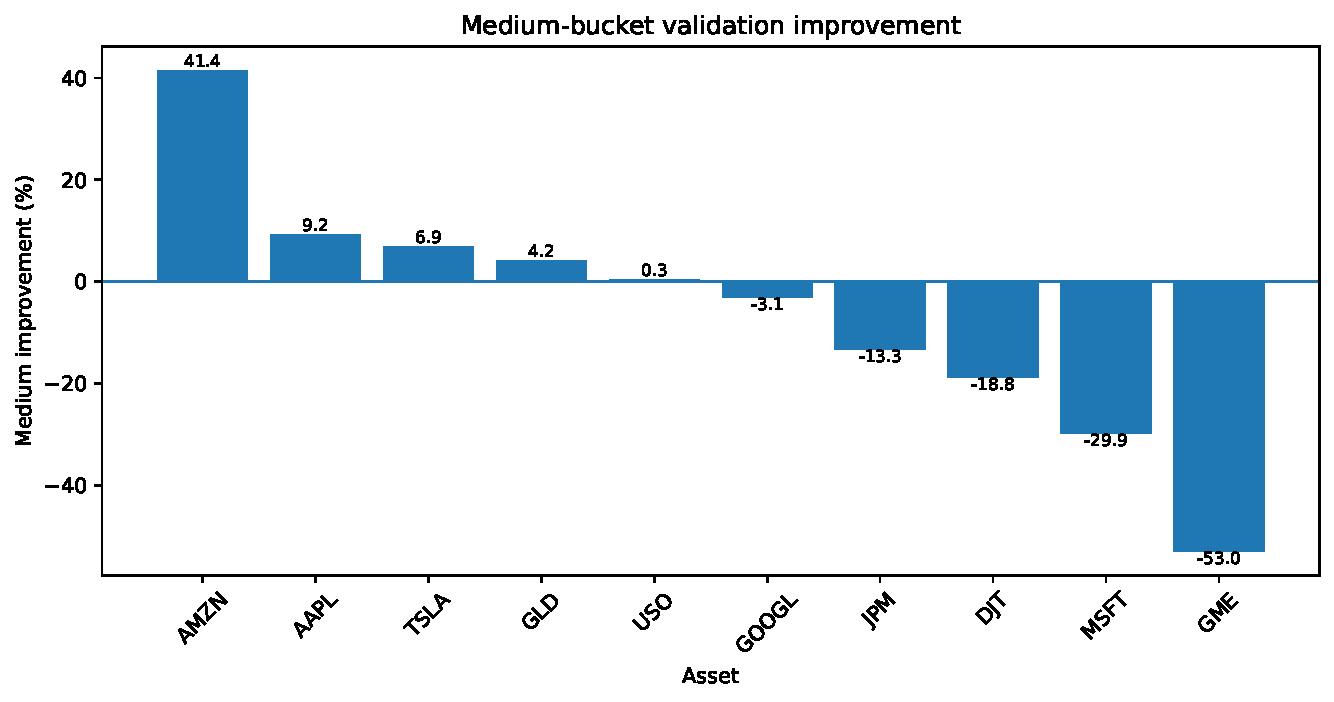
\includegraphics[width=0.85\textwidth]{fig7_2_medium_improvement.pdf}
\caption{Medium-bucket validation improvement of TFBS relative to Black--Scholes.}
\label{fig:medium_improvement}
\end{figure}

Medium bucket에서 가장 뚜렷한 improvement를 보인 asset은 AMZN이다. AMZN의 Medium improvement는 약 $41.4\%$로, 이번 실험에서 가장 강한 medium-maturity positive case이다. AAPL, TSLA, GLD, USO는 Medium bucket에서 양의 improvement를 보였지만 그 크기는 상대적으로 작다. 반면 MSFT, GOOGL, JPM, GME, DJT는 Medium bucket에서 negative result를 보였다.

따라서 본 실험 결과는 TFBS의 medium-maturity advantage가 일부 asset에서 나타나지만, 그 효과는 asset-specific하다는 것이다. 즉, medium maturity라는 구간 자체가 TFBS improvement를 자동으로 보장하지는 않는다.

\section{Validation RMSE Term Structures}

Figure~\ref{fig:selected_rmse_term_structures}는 대표적인 네 개의 asset에 대한 validation RMSE term structure를 보여준다. 여기서는 AMZN, MSFT, TSLA, GLD를 선택하였다. AMZN은 blue-chip positive case, MSFT는 blue-chip negative case, TSLA는 high-attention group의 moderate positive case, GLD는 commodity-linked ETF의 weak positive 또는 near-neutral case를 대표한다.

\begin{figure}[htbp]
\centering
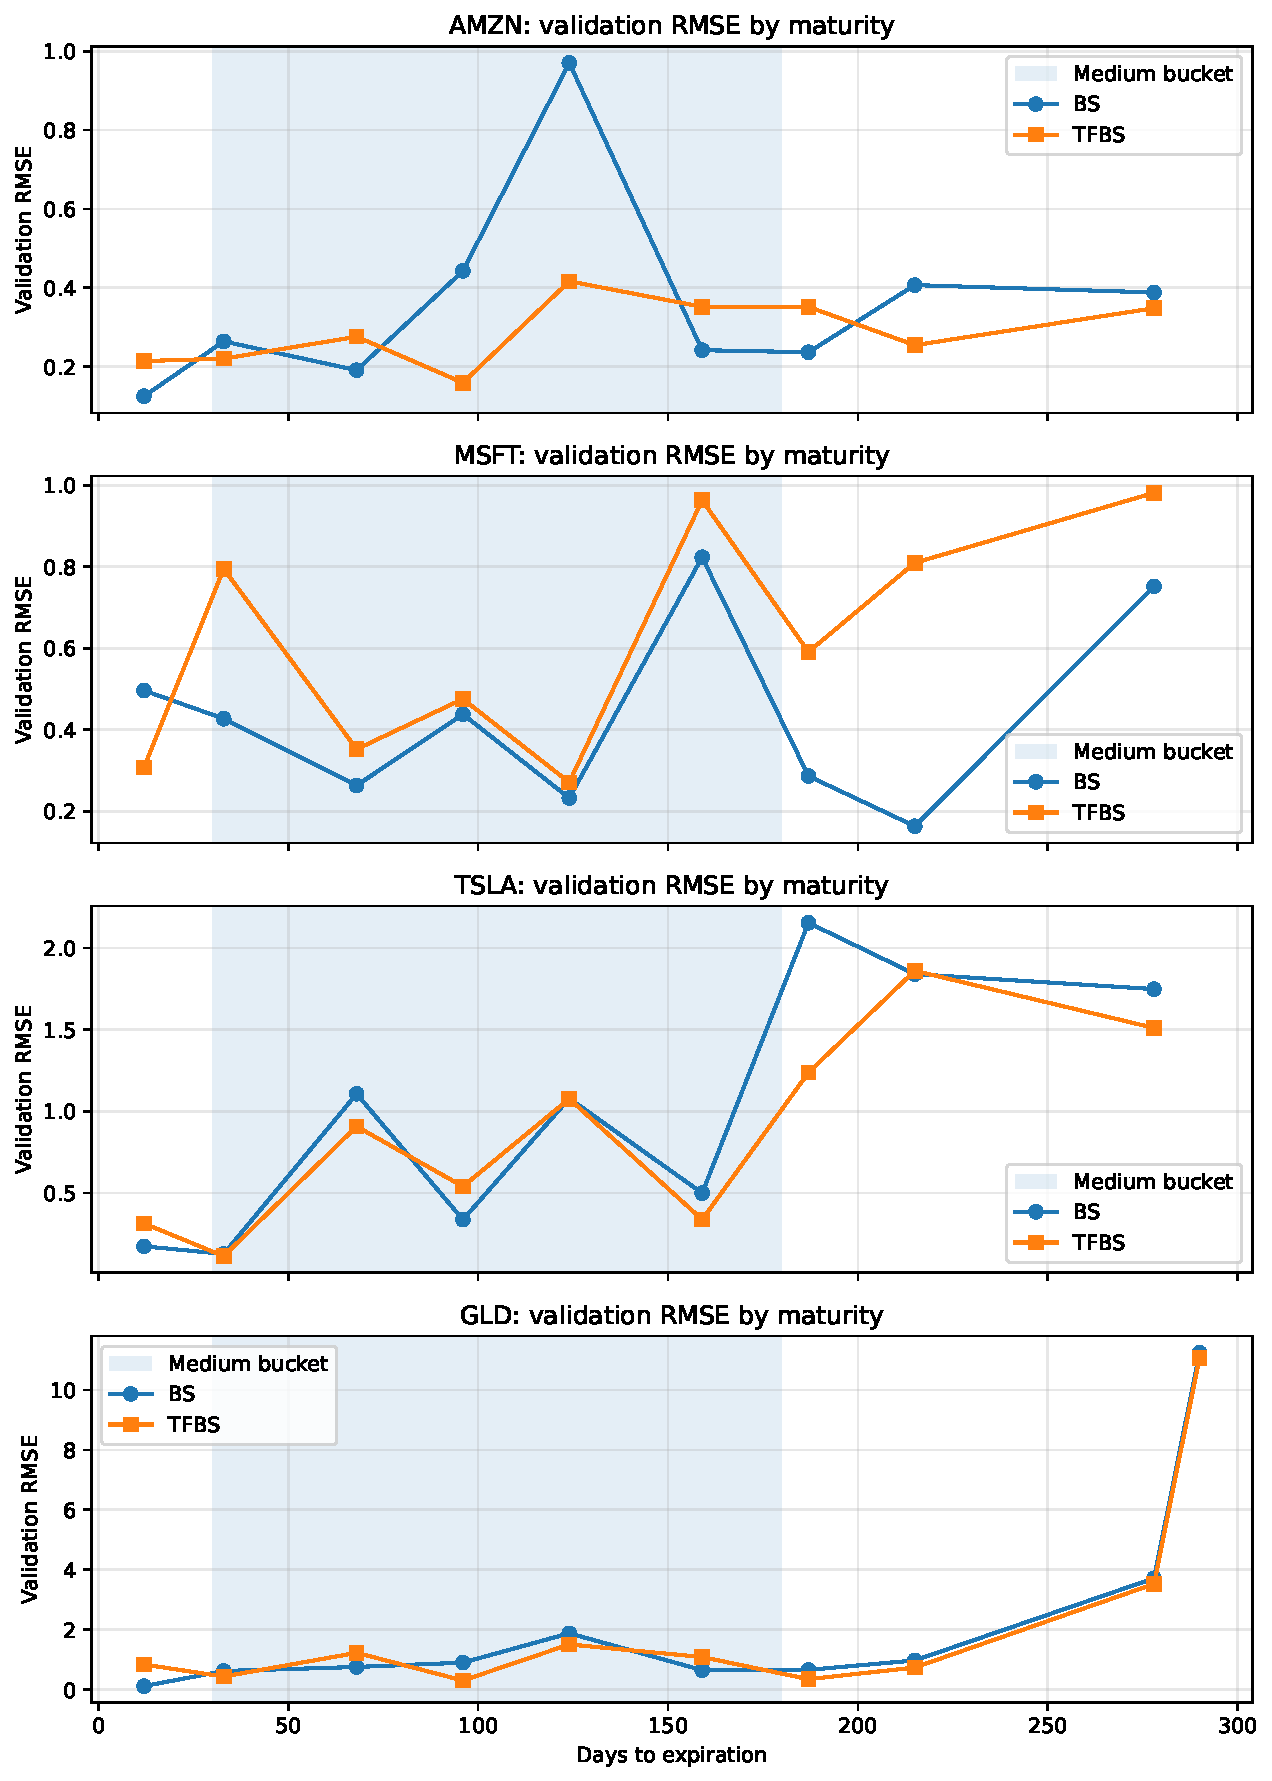
\includegraphics[width=0.9\textwidth]{fig7_3_selected_rmse_term_structures.pdf}
\caption{Validation RMSE term structures for selected representative assets. The shaded region denotes the medium-maturity bucket.}
\label{fig:selected_rmse_term_structures}
\end{figure}

AMZN의 term structure에서는 medium 및 long maturity region에서 TFBS RMSE가 Black--Scholes RMSE보다 낮게 나타난다. 이는 AMZN의 positive improvement가 특정 single bucket artifact가 아니라 maturity term structure 전반에서 관찰되는 패턴임을 보여준다. 반대로 MSFT는 medium 및 long maturity에서 TFBS RMSE가 높게 나타나며, 이는 MSFT의 negative bucket-level result와 일치한다.

TSLA는 short maturity에서는 TFBS가 불리하지만, medium 및 long maturity에서는 TFBS가 일부 improvement를 보인다. 이는 high-attention asset에서 TFBS가 완전히 실패하는 것은 아니지만, maturity별 결과가 안정적이지 않을 수 있음을 보여준다. GLD는 전체적으로 두 model의 RMSE 차이가 크지 않으며, commodity-linked ETF에서 TFBS의 추가 설명력이 제한적일 수 있음을 시사한다.

\section{TFBS Parameter Signatures}

Validation performance만으로는 TFBS가 어떤 방식으로 option surface를 설명하는지 알기 어렵다. 따라서 본 절에서는 TFBS calibration에서 얻어진 $\alpha$와 $\lambda$의 asset별 structure를 살펴본다. Figure~\ref{fig:parameter_signatures}는 각 asset의 calibrated fractional order $\widehat{\alpha}$와 maturity bucket별 average tempering parameter $\widehat{\lambda}$를 보여준다.

\begin{figure}[htbp]
\centering
\begin{subfigure}{0.48\textwidth}
\centering
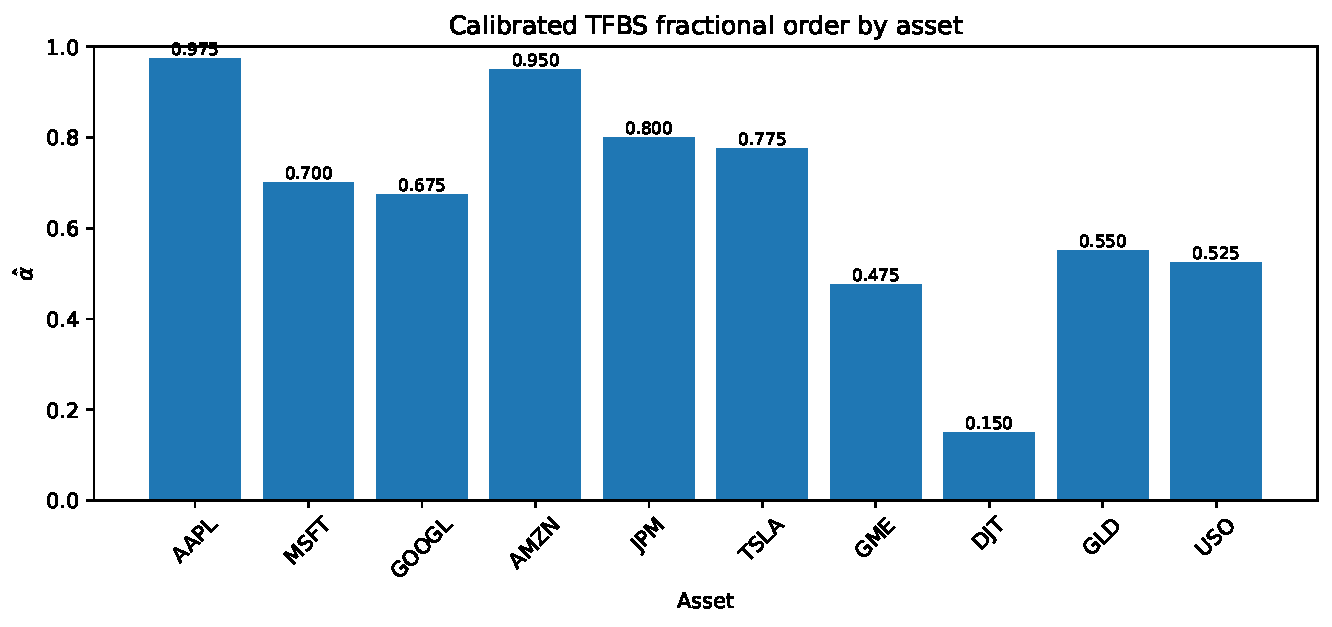
\includegraphics[width=\textwidth]{fig7_4a_alpha_by_asset.pdf}
\caption{Calibrated fractional order.}
\end{subfigure}
\hfill
\begin{subfigure}{0.48\textwidth}
\centering
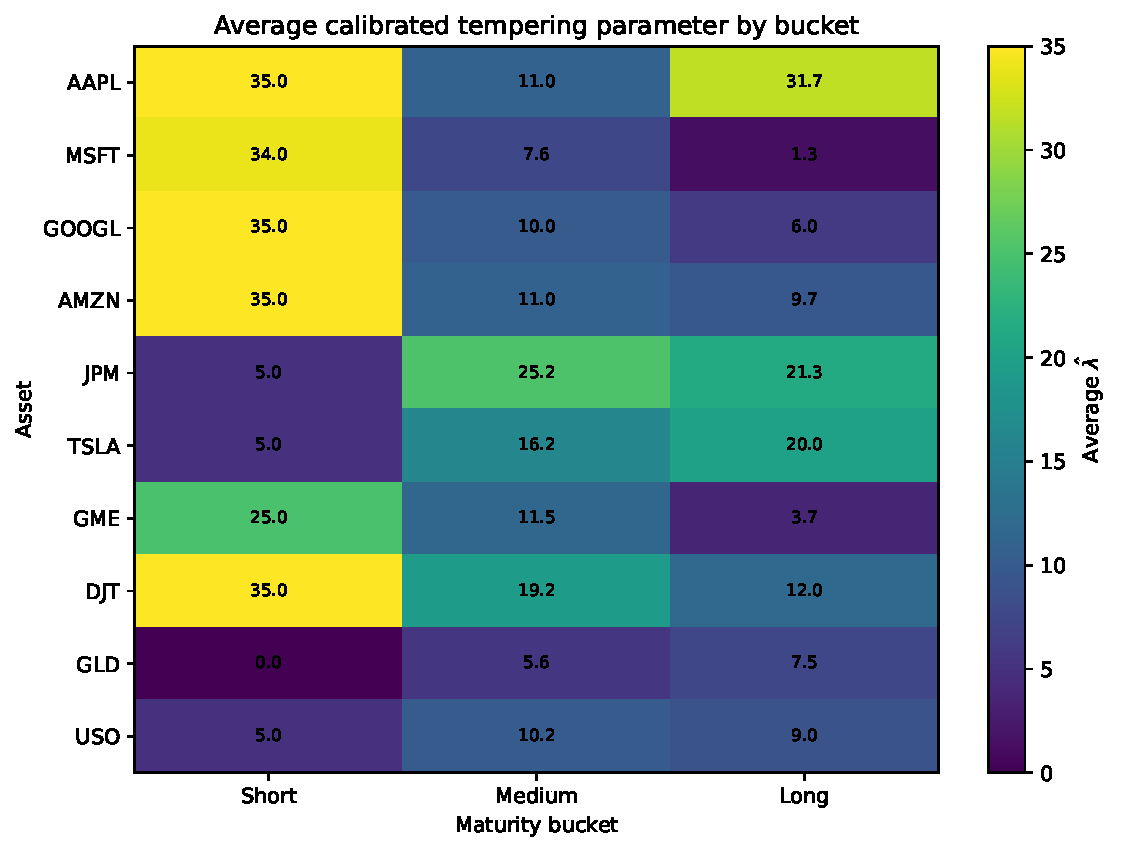
\includegraphics[width=\textwidth]{fig7_4b_lambda_bucket_heatmap.pdf}
\caption{Average tempering parameter by maturity bucket.}
\end{subfigure}
\caption{TFBS parameter signatures across assets.}
\label{fig:parameter_signatures}
\end{figure}

Calibrated $\widehat{\alpha}$는 asset별로 상당히 다르게 나타난다. AAPL과 AMZN은 $\widehat{\alpha}$가 각각 $0.975$와 $0.950$으로 1에 가까운 값을 보인다. 이는 이 두 asset에서 TFBS가 강한 fractional memory보다는 classical time derivative에 가까운 weak fractional correction을 사용한다는 의미로 해석할 수 있다. 반면 GME, GLD, USO는 상대적으로 낮은 $\widehat{\alpha}$를 보이며, DJT는 매우 낮은 $\widehat{\alpha}$를 갖는다. 그러나 낮은 $\alpha$가 반드시 좋은 validation performance로 이어지지는 않는다. 예를 들어 GME는 낮은 $\alpha$를 보이지만 overall validation performance는 negative이다. 따라서 $\alpha$만으로 TFBS의 성능을 설명할 수는 없다.

Tempering parameter $\lambda$ 역시 asset과 maturity bucket에 따라 크게 달라진다. 일부 asset에서는 높은 $\lambda$ 값이 반복적으로 선택된다. 이는 TFBS가 persistent long memory보다는 빠르게 감쇠하는 strongly tempered memory를 선호할 수 있음을 시사한다. 그러나 $\lambda$가 높은 값으로 자주 추정되는 경우에는 grid boundary effect의 가능성을 고려해야 하므로, parameter interpretation은 조심스럽게 이루어져야 한다.

특히 AMZN은 strong positive case임에도 $\alpha$가 1에 가깝다. 이는 TFBS의 개선이 반드시 강한 fractional memory에서만 발생하는 것이 아니라, 약한 fractional correction과 tempering structure의 조합에서도 나타날 수 있음을 보여준다. 반대로 GME와 DJT는 낮은 $\alpha$ 또는 높은 tempering parameter를 보이지만 validation improvement는 안정적이지 않다. 따라서 TFBS parameter는 개별적으로 해석하기보다, validation performance와 함께 memory-tempering signature로 해석하는 것이 적절하다.

\section{Summary of Empirical Findings}

본 장의 cross-asset empirical results는 다음과 같이 요약할 수 있다.

첫째, TFBS model은 Black--Scholes benchmark를 모든 asset과 maturity bucket에서 보편적으로 개선하지 않는다. 일부 asset에서는 positive improvement가 나타나지만, 다른 asset에서는 weak, mixed, 또는 negative result가 나타난다.

둘째, medium maturity bucket에서 TFBS가 항상 우월하다는 결론은 성립하지 않는다. AMZN은 medium bucket에서 가장 강한 positive case이지만, MSFT, GME, DJT, JPM 등에서는 medium bucket에서 negative result가 나타난다. 따라서 medium-maturity advantage는 universal property가 아니라 asset-specific phenomenon으로 해석해야 한다.

셋째, blue-chip equities 내부에서도 결과는 이질적이다. AMZN은 strong positive case이고, MSFT는 negative case이며, GOOGL은 near-neutral case이다. JPM은 medium이 아니라 long maturity에서 improvement가 나타나는 long-driven case이다. 따라서 liquid blue-chip 여부 자체가 TFBS performance를 결정하지 않는다.

넷째, high-attention 또는 event-driven equities에서는 결과가 불안정하다. TSLA는 medium 및 long maturity에서 moderate improvement를 보이지만, GME와 DJT는 negative validation performance를 보인다. 이는 event risk, speculative demand, liquidity condition이 option surface를 지배할 경우 TFBS의 memory-tempering structure가 안정적으로 generalize되지 않을 수 있음을 시사한다.

다섯째, commodity-linked ETFs에서는 TFBS의 추가 설명력이 약하다. GLD와 USO는 전체적으로 weak 또는 near-neutral result를 보이며, commodity cycle과 macro factor가 option surface를 더 크게 지배할 가능성을 시사한다.

결론적으로 본 장의 결과는 TFBS model을 universal pricing formula로 해석하기보다, 특정 option surface에 finite-horizon memory structure가 존재하는지를 진단하는 memory-diagnostic pricing model로 해석하는 것이 적절함을 보여준다. 다음 장에서는 이러한 asset-dependent performance의 차이를 설명할 수 있는 candidate drivers를 논의한다.




















\chapter{Candidate Drivers of Asset-Dependent Performance}

\section{Overview}

제7장에서 확인한 cross-asset empirical results는 TFBS model이 Black--Scholes benchmark를 모든 자산과 모든 만기에서 일괄적으로 개선하지 않는다는 점을 보여준다. 일부 asset에서는 medium 또는 long maturity bucket에서 validation RMSE가 낮아졌지만, 다른 asset에서는 improvement가 약하거나 음수로 나타났다. 따라서 TFBS의 성능은 universal model performance라기보다 maturity-dependent and asset-specific performance로 해석하는 것이 적절하다.

본 장에서는 이러한 성능 차이를 설명할 수 있는 candidate drivers를 논의한다. 본 장에서 다루는 주요 candidate drivers는 다음과 같다.
\[
\begin{aligned}
&\text{(i) stable finite-horizon memory structure},\\
&\text{(ii) short-maturity noise and payoff nonlinearity},\\
&\text{(iii) option-surface smoothness and generalization},\\
&\text{(iv) high-attention and event-driven instability},\\
&\text{(v) commodity and macro-factor dominance},\\
\end{aligned}
\]

이러한 요인들은 asset과 maturity bucket에 따라 동시에 작용할 수 있다.

\section{Stable Finite-Horizon Memory Structure}

TFBS model이 잘 작동하기 위한 가장 중요한 조건은 option surface에 안정적인 finite-horizon memory structure가 존재하는 것이다. TFBS의 memory kernel은
\[
K_{\alpha,\lambda}(u)
=
e^{-\lambda u}u^{-\alpha}
\]
로 주어진다. 여기서 \(\alpha\)는 fractional memory의 shape을 나타내고, \(\lambda\)는 memory effect가 time lag에 따라 얼마나 빠르게 감쇠하는지를 조절한다. 따라서 TFBS는 단순히 과거 정보의 영향이 오래 지속된다고 가정하는 model이 아니라, 과거 정보의 영향이 일정한 horizon 안에서 점차 약해지는 구조를 표현할 수 있다.

제7장의 결과에서 positive improvement가 나타나는 asset은 이러한 finite-horizon memory structure가 validation strike로 어느 정도 일반화되는 경우로 해석할 수 있다. 예를 들어 AMZN은 medium bucket에서 가장 뚜렷한 positive improvement를 보였다. 이는 AMZN option surface에서 TFBS가 calibration strike에서 추정한 memory-tempering structure를 validation strike에도 비교적 안정적으로 적용할 수 있었음을 시사한다.

그러나 이러한 구조가 모든 asset에서 나타나는 것은 아니다. AAPL, GOOGL, MSFT, JPM과 같은 같은 blue-chip group 안에서도 결과가 서로 다르게 나타났다. 따라서 liquid blue-chip 여부 자체가 TFBS의 성능을 결정한다고 보기는 어렵다. 중요한 것은 해당 option surface가 maturity와 strike 방향으로 TFBS의 memory-tempering structure를 안정적으로 반영할 수 있는지 여부이다.

\section{Short-Maturity Noise and Payoff Nonlinearity}

Short maturity bucket에서는 대부분의 asset에서 TFBS의 performance가 불안정하게 나타난다. 이는 short maturity options가 model-implied memory structure보다 market microstructure noise와 payoff nonlinearity에 더 크게 영향을 받을 수 있기 때문이다.

첫째, 만기까지 남은 시간이 짧을수록 call payoff \((S-K)^+\)의 kink가 가격에 더 강하게 반영된다. 특히 at-the-money 부근에서는 gamma sensitivity가 커지므로, 작은 기초자산 가격 변화나 quote 변화가 option price에 크게 반영될 수 있다. 이러한 특성은 smooth한 PDE-based pricing model의 calibration을 어렵게 만든다.

둘째, short maturity options는 bid--ask spread, 거래량 부족, stale lastPrice와 같은 market microstructure effects에 민감하다. 본 논문의 data source는 public option chain data이며, 일부 실험에서는 bid--ask midpoint 대신 last transaction price를 market price proxy로 사용한다. LastPrice는 마지막 체결 시점의 가격이므로, 현재 quote와 괴리될 수 있다. 이 문제는 특히 short maturity options에서 validation RMSE를 크게 흔들 수 있다.

셋째, short bucket의 표본 수 자체가 적은 경우가 많다. 본 실험에서는 target DTE 방식으로 maturity를 선택하지만, 실제 option chain에서 short bucket에 들어가는 expiry 수는 제한적일 수 있다. 따라서 short bucket의 improvement percentage는 하나 또는 두 개의 expiry에 의해 크게 좌우될 수 있다. 이러한 이유로 본 논문에서는 short bucket의 결과를 주요 결론으로 사용하기보다, medium 및 long bucket의 결과와 함께 보조적으로 해석한다.

\section{Option-Surface Smoothness and Generalization}

TFBS model은 Black--Scholes model보다 더 많은 parameters를 포함한다. 따라서 calibration set에서는 더 낮은 error를 만들 수 있지만, 이 improvement가 validation set에서도 유지되려면 option surface의 구조가 충분히 smooth하고 stable해야 한다. 즉, calibration strike에서 추정한 \((\alpha,\sigma,\lambda)\) structure가 validation strike로 일반화되어야 한다.

이 관점에서 TFBS의 성능 차이는 option-surface smoothness와 관련될 수 있다. 어떤 asset에서는 strike와 maturity 방향으로 option prices가 비교적 매끄럽게 변하고, TFBS가 포착한 memory-tempering structure가 validation strike에서도 유지된다. 이런 경우 TFBS는 Black--Scholes benchmark보다 낮은 validation RMSE를 보일 수 있다. 반면 option surface가 특정 strike나 maturity에서 불규칙하게 움직이면, TFBS의 추가 parameter는 calibration set에는 잘 맞지만 validation set에는 일반화되지 않을 수 있다.

제7장의 blue-chip results는 이 점을 잘 보여준다. 같은 liquid blue-chip equities 안에서도 AMZN은 medium bucket에서 strong positive case로 나타났지만, MSFT는 medium 및 long bucket에서 negative performance를 보였다. GOOGL은 거의 neutral한 결과를 보였고, JPM은 medium이 아니라 long bucket에서 improvement가 주로 나타났다. 이는 TFBS performance가 asset class label만으로 결정되는 것이 아니라, 각 asset의 option surface가 갖는 smoothness와 maturity structure에 크게 의존함을 시사한다.

\section{High-Attention and Event-Driven Instability}

High-attention 또는 event-driven equities에서는 TFBS의 성능이 더 불안정하게 나타날 수 있다. TSLA, GME, DJT와 같은 자산은 retail attention, speculative demand, event risk, jump-like movement의 영향을 크게 받을 수 있다. 이러한 요인들은 smooth memory kernel보다는 갑작스러운 price movement나 sentiment shock의 형태로 option price에 반영될 수 있다.

TSLA의 경우 medium 및 long bucket에서 moderate improvement가 나타났지만, short bucket에서는 negative performance가 나타났다. 이는 TSLA option surface에서 TFBS가 일부 maturity region에서는 Black--Scholes보다 낮은 validation error를 보일 수 있지만, 그 structure가 모든 maturity에 걸쳐 안정적으로 유지되지는 않음을 의미한다.

GME와 DJT는 더 불안정한 결과를 보인다. 이들 asset에서는 event risk와 speculative demand가 option price를 지배할 가능성이 크다. 이러한 경우 TFBS의 memory-tempering structure가 validation strike로 안정적으로 일반화되기 어렵다. 특히 high-attention assets에서 추정된 \(\lambda\)가 큰 값으로 나타나는 경우, 이는 persistent long memory라기보다 빠르게 감쇠하는 event-driven memory 또는 attention effect를 model이 포착하려는 것으로 해석할 수 있다. high-attention group의 결과는 TFBS의 한계와 parameter instability를 보여주는 중요한 comparison group으로 볼 수 있다.

\section{Commodity and Macro-Factor Dominance}

Commodity 또는 spot-linked ETFs에서는 equity options와 다른 요인이 option surface를 지배할 수 있다. GLD와 USO는 각각 금 및 원유 관련 market factor와 연결된 ETF이다. 이들 자산의 option prices는 개별 기업의 earnings나 firm-specific news보다는 commodity cycle, macro factor, dollar movement, inflation expectation, futures market structure 등에 더 민감할 수 있다.

제7장의 결과에서 GLD와 USO는 TFBS의 improvement가 약하거나 거의 neutral한 모습을 보였다. 이는 commodity-linked ETFs의 option surface에서는 finite-horizon memory kernel만으로 설명되는 부분이 제한적일 수 있음을 시사한다. 특히 long maturity options에서는 macroeconomic uncertainty와 commodity-specific risk가 강하게 작용할 수 있으므로, 단순한 memory-tempering structure가 validation performance를 크게 개선하지 못할 수 있다.

이 결과는 TFBS model이 equity option surface에서는 일부 설명력을 가질 수 있지만, commodity-linked ETF option surface에서는 그 효과가 약해질 수 있음을 보여준다. 따라서 asset class에 따라 TFBS의 usefulness가 달라질 수 있다는 본 논문의 asset-specific interpretation과 일관된다.

\section{Summary of Candidate Drivers}

Table~\ref{tab:candidate_drivers}는 본 장에서 논의한 candidate drivers를 요약한다. 이 표는 각 driver가 어떤 empirical pattern과 연결되는지, 그리고 어떤 해석을 가능하게 하는지 정리한 것이다.

\begin{table}[htbp]
\centering
\small
\begin{tabular}{p{0.22\textwidth}p{0.30\textwidth}p{0.34\textwidth}}
\toprule
Candidate driver & Expected empirical pattern & Interpretation \\
\midrule
Stable finite-horizon memory
&
Positive validation improvement in medium or long maturity; moderate and interpretable \(\lambda\)
&
TFBS captures a memory structure that generalizes from calibration strikes to validation strikes.
\\
\midrule
Short-maturity noise
&
Unstable or negative short-bucket improvement
&
Payoff kink, high gamma sensitivity, bid--ask noise, and stale price effects dominate short maturities.
\\
\midrule
Option-surface smoothness
&
Improvement differs even within the same asset class
&
Asset class label alone is insufficient; the smoothness and stability of each option surface matter.
\\
\midrule
Event-driven instability
&
High or unstable \(\lambda\), mixed validation performance in high-attention assets
&
TFBS may capture short-lived event or attention effects rather than stable long memory.
\\
\midrule
Commodity and macro factors
&
Weak or near-neutral improvement for commodity-linked ETFs
&
Macro and commodity-specific risk may dominate the option surface.
\\
\\
\bottomrule
\end{tabular}
\caption{Candidate drivers of asset-dependent TFBS performance.}
\label{tab:candidate_drivers}
\end{table}

Overall, the cross-asset differences should not be interpreted as evidence that TFBS is universally superior or inferior to Black--Scholes. Rather, they suggest that TFBS is useful when the option surface contains a stable finite-horizon memory structure that can be captured by \(\alpha\) and \(\lambda\). When option prices are dominated by short-maturity noise, event-driven jumps, or macro-commodity factors, the additional flexibility of TFBS may not translate into improved validation performance.

따라서 본 논문의 핵심 해석은 다음과 같다. TFBS model은 universal pricing formula가 아니라, option surface에 memory-tempering structure가 존재하는지를 확인하는 diagnostic pricing model이다. 다음 장에서는 이러한 해석을 바탕으로 grid sensitivity, price source, numerical resolution, maturity bucket definition, calibration--validation split 등 robustness checks와 model limitations를 정리한다.






















\chapter{Robustness Checks and Limitations}

\section{Overview}

제7장에서는 여러 기초자산에 대해 TFBS model과 Black--Scholes benchmark의 validation performance를 비교하였고, 제8장에서는 그 차이를 설명할 수 있는 candidate drivers를 논의하였다. 본 장에서는 이러한 empirical results를 해석할 때 고려해야 할 robustness issues와 limitations를 정리한다.

TFBS의 performance는 maturity bucket, asset class, option surface의 구조, market price proxy, parameter grid 등에 따라 달라진다. 따라서 empirical results는 특정 data source, filtering rule, parameter grid, numerical resolution, calibration--validation split에 조건부인 결과로 해석해야 한다.

본 장에서는 다음 다섯 가지 측면을 중심으로 robustness와 한계를 논의한다.
\[
\begin{aligned}
&\text{(i) parameter grid sensitivity},\\
&\text{(ii) market price proxy and price-source limitation},\\
&\text{(iii) numerical resolution},\\
&\text{(iv) maturity bucket and validation split},\\
&\text{(v) model specification limitations}.
\end{aligned}
\]
이러한 논의는 본 연구의 empirical findings를 과장하지 않고, TFBS model을 어떤 범위 안에서 해석해야 하는지를 명확히 하기 위한 것이다.

\section{Grid Sensitivity and Parameter Boundary}

TFBS model은 fractional order $\alpha$, volatility parameter $\sigma$, tempering parameter $\lambda$를 포함한다. 따라서 calibration result는 parameter grid의 range와 resolution에 영향을 받을 수 있다. 본 논문에서는 계산량을 줄이기 위해 coarse-to-fine grid strategy를 사용하였다. 먼저 coarse grid에서 대략적인 parameter region을 탐색한 뒤, 각 maturity별 coarse optimum 주변에서 local fine grid를 구성하였다.

그러나 finite grid search에는 몇 가지 한계가 있다. 첫째, true optimum이 grid point 사이에 위치할 수 있다. 이 경우 estimated parameter는 가장 가까운 grid point로 선택되며, parameter estimates에는 discretization error가 포함될 수 있다. 둘째, 최적 parameter가 grid boundary 근처에서 반복적으로 선택되면, 실제 optimum이 grid 밖에 있을 가능성을 배제할 수 없다. 특히 $\lambda$가 높은 값으로 반복적으로 선택되는 경우, TFBS가 strongly tempered memory를 선호한다는 해석과 동시에, $\lambda$ grid가 충분히 넓지 않을 수 있다는 가능성을 함께 고려해야 한다.

본 연구의 결과에서도 일부 assets에서 높은 $\lambda$ values가 선택된다. 이는 해당 option surface에서 persistent long memory보다 빠르게 감쇠하는 memory structure가 더 적합하다는 해석과 일관될 수 있다. 그러나 동시에 high-\(\lambda\) estimates는 parameter boundary effect를 포함할 수 있으므로, $\lambda$의 수치값 자체를 실제 시장의 memory horizon으로 직접 해석하는 것은 조심해야 한다.

따라서 본 논문에서 추정된 $\alpha$와 $\lambda$는 structural physical parameters가 아니라, finite grid calibration을 통해 얻어진 model-implied memory signature로 해석한다. 즉, parameter의 절대값보다 중요한 것은 각 asset과 maturity bucket에서 TFBS가 어떤 direction의 memory-tempering structure를 선택하는지, 그리고 그것이 validation RMSE improvement와 함께 나타나는지이다.

\section{Market Price Proxy and Price-Source Limitation}

Option pricing model을 empirical data에 적용할 때 가장 중요한 문제 중 하나는 market price의 정의이다. 이상적으로는 bid--ask midpoint를 사용하는 것이 바람직하다. 그러나 public option chain data에서는 모든 contract에 대해 신뢰할 수 있는 bid와 ask가 제공되지 않거나, bid 또는 ask가 0으로 표시되는 경우가 있다. 이러한 경우에는 last transaction price, 즉 lastPrice를 market price proxy로 사용할 수밖에 없다.

LastPrice는 실제로 체결된 가격이라는 장점이 있지만, 마지막 체결 시점이 현재 관측 시점과 다를 수 있다는 문제가 있다. 따라서 lastPrice는 stale price일 수 있으며, 특히 거래량이 적은 option이나 short maturity option에서 이 문제가 더 심각할 수 있다. Stale price는 validation RMSE를 크게 흔들 수 있으므로, model performance의 일부는 pricing model의 구조적 차이뿐 아니라 data noise를 반영할 수 있다.

본 논문의 empirical results는 이러한 public data limitation을 고려하여 해석해야 한다. TFBS가 특정 asset에서 Black--Scholes보다 낮은 validation RMSE를 보였다고 하더라도, 그 결과가 bid--ask midpoint 기반 data에서도 동일하게 유지되는지는 별도의 robustness check가 필요하다. 반대로 TFBS가 특정 asset에서 나쁜 performance를 보였을 경우에도, 그 원인이 model structure 자체인지, stale lastPrice 또는 liquidity 문제인지 완전히 분리하기 어렵다.

따라서 본 연구의 empirical analysis는 public option data에 기반한 preliminary validation study로 이해하는 것이 적절하다. 향후 연구에서는 보다 고품질의 quote-level data를 사용하여 bid--ask midpoint, trade price, quote timestamp, volume, open interest 등을 함께 고려한 robustness analysis가 필요하다.

\section{Numerical Resolution}

TFBS option price는 closed-form formula가 아니라 finite difference scheme을 통해 계산된다. 따라서 numerical resolution, 즉 time grid size와 space grid size가 pricing result에 영향을 줄 수 있다. 본 논문에서는 time-to-maturity direction을 $N$개의 time steps로 나누고, underlying price direction을 $M$개의 spatial intervals로 나누어 TFBS PDE를 이산화하였다.

Numerical resolution이 너무 낮으면 discretization error가 커질 수 있다. 특히 fractional derivative는 과거 time increments의 weighted history를 포함하므로, time discretization이 충분히 세밀하지 않으면 memory term approximation이 부정확해질 수 있다. 반대로 $M$과 $N$을 지나치게 크게 설정하면 각 parameter combination마다 PDE solver를 반복적으로 실행해야 하므로 계산량이 크게 증가한다.

본 논문에서는 computational feasibility를 고려하여 moderate resolution을 사용하였다. 또한 parameter search에서 coarse grid와 final grid의 PDE resolution을 구분하여, initial scan에서는 상대적으로 낮은 resolution을 사용하고 final calibration에서는 더 높은 resolution을 사용하였다. 이는 계산량과 numerical accuracy 사이의 trade-off를 반영한 설계이다.

다만 본 연구는 full convergence analysis를 수행하지 않는다. 즉, $M,N\to\infty$에서 numerical solution이 theoretical TFBS solution으로 수렴한다는 엄밀한 numerical analysis를 본문의 주요 목표로 삼지 않는다. 본 논문의 목적은 TFBS PDE를 이용한 empirical validation framework를 구성하고, 여러 asset과 maturity bucket에서 model performance를 비교하는 데 있다. 따라서 numerical resolution에 따른 결과 변화는 limitation으로 남으며, 향후 연구에서 보다 체계적인 convergence and stability analysis가 필요하다.

\section{Maturity Bucket Sensitivity}

본 논문은 maturity-dependent performance를 분석하기 위해 short, medium, long maturity buckets를 사용한다. 기본적인 구분은 다음과 같다.
\[
\text{Short}: T\le 30\ \text{days},
\]
\[
\text{Medium}: 30<T\le 180\ \text{days},
\]
\[
\text{Long}: T>180\ \text{days}.
\]
이 구분은 option market에서 자주 사용되는 직관적인 maturity segmentation에 기반하지만, 절대적인 기준은 아니다. 예를 들어 medium maturity의 상한을 180 days로 둘지, 210 days로 둘지에 따라 일부 expiry가 Medium bucket에서 Long bucket으로 이동할 수 있다.

따라서 medium-maturity advantage를 해석할 때에는 bucket boundary의 임의성을 고려해야 한다. 어떤 asset에서 improvement가 180-day 근처의 expiry에 집중되어 있다면, bucket definition을 약간 변경했을 때 Medium bucket result가 달라질 수 있다. 반대로 improvement가 여러 medium expiry에 걸쳐 안정적으로 나타난다면, bucket boundary에 덜 민감한 결과로 볼 수 있다.

본 논문에서 maturity buckets는 theory-driven classification이라기보다 empirical grouping으로 사용된다. 즉, short, medium, long buckets는 model performance를 요약하기 위한 분석 단위이다. 따라서 결과 해석에서는 각 bucket의 pooled RMSE뿐 아니라 expiry-level results도 함께 고려하는 것이 중요하다. 특히 제7장에서 제시한 RMSE term structure는 bucket-level average가 개별 maturity에서 어떻게 나타나는지 확인하기 위한 보조적 역할을 한다.

\section{Calibration--Validation Split Sensitivity}

TFBS model은 Black--Scholes benchmark보다 더 많은 parameters를 포함하므로, in-sample calibration error만으로 model을 비교하는 것은 적절하지 않다. 본 논문에서는 이를 보완하기 위해 각 maturity별 strike set을 calibration set과 validation set으로 나누었다. 기본 split은 strike를 오름차순으로 정렬한 뒤 alternating split을 적용하는 방식이다.

이 방식의 장점은 calibration set과 validation set이 모두 in-the-money, near-the-money, out-of-the-money strike를 어느 정도 포함할 수 있다는 점이다. 그러나 validation result는 split 방식에 따라 달라질 수 있다. 예를 들어 특정 maturity에서 validation set에 포함된 strike가 stale price 또는 abnormal quote를 포함하고 있다면, validation RMSE는 크게 왜곡될 수 있다.

또한 각 maturity에서 사용되는 strike 수가 많지 않기 때문에, validation set의 크기도 제한적이다. 본 연구의 기본 설계에서는 각 expiry당 near-the-money strikes를 일정 개수 선택하고, 그중 일부를 calibration, 나머지를 validation으로 사용한다. 이 경우 maturity별 validation RMSE는 소수의 option contracts에 의해 영향을 받을 수 있다.

따라서 본 논문의 validation result는 split-specific result로 이해해야 한다. 보다 강한 robustness를 확보하기 위해서는 reversed alternating split, random repeated split, 또는 cross-validation-style strike split을 사용할 수 있다. 본 논문에서는 alternating split을 통해 in-sample fitting과 out-of-sample validation을 구분하는 기본 framework를 제시하지만, split sensitivity는 향후 연구에서 더 체계적으로 다룰 수 있는 부분이다.

\section{Model Specification Limitations}

본 논문의 TFBS model은 Black--Scholes spatial operator를 유지하면서 time derivative를 tempered fractional derivative로 대체한 reduced-form PDE model이다. 이 접근은 Black--Scholes benchmark와 비교 가능한 구조를 유지하면서 time-nonlocal memory effect를 도입할 수 있다는 장점이 있다. 그러나 model specification 측면에서 몇 가지 한계를 가진다.

첫째, 본 논문은 full no-arbitrage stochastic foundation을 제공하지 않는다. Fractional Brownian motion이나 long-memory process를 기초자산 dynamics에 직접 도입할 경우, no-arbitrage condition과 관련된 복잡한 문제가 발생할 수 있다. 본 연구는 이러한 문제를 해결하기보다, option surface에 finite-horizon memory structure가 존재하는지를 확인하기 위한 reduced-form fractional PDE approach를 사용한다.

둘째, 본 논문의 PDE는 European-style call option pricing problem을 기반으로 한다. 그러나 미국 시장에서 거래되는 equity options와 ETF options는 일반적으로 American-style exercise feature를 갖는다. 본 연구에서는 call options에 초점을 두고, Black--Scholes benchmark와 TFBS model을 동일한 조건에서 비교하므로 relative validation performance가 주된 분석 대상이다. 그럼에도 불구하고 absolute pricing accuracy를 해석할 때에는 early exercise feature의 영향을 고려해야 한다.

셋째, interest rate와 dividend yield는 단순화하여 처리된다. 실제 option price는 term structure of interest rates, discrete dividends, borrow costs, transaction costs, liquidity premium 등 다양한 요인의 영향을 받을 수 있다. 본 논문은 이러한 모든 요인을 modeling하는 것을 목표로 하지 않고, fractional time dynamics가 Black--Scholes benchmark에 비해 validation pricing error를 개선할 수 있는지에 초점을 둔다.

넷째, TFBS model은 volatility smile이나 jump risk를 직접적으로 model하지 않는다. TFBS의 추가 flexibility는 time direction의 fractional memory와 tempering에서 비롯된다. 따라서 event-driven assets나 jump-like movement가 강한 assets에서는 TFBS의 memory-tempering structure만으로 option surface를 충분히 설명하지 못할 수 있다. 이는 GME, DJT와 같은 high-attention assets에서 negative 또는 unstable validation performance가 나타나는 것과 일관적인 해석을 제공한다.

\section{Interpretation of Empirical Findings}

위의 robustness issues와 limitations를 고려하면, 본 논문의 empirical findings는 다음과 같이 해석하는 것이 적절하다.

첫째, TFBS가 어떤 asset에서 positive validation improvement를 보였다고 해서, 그 model이 해당 asset의 true pricing mechanism을 정확히 설명한다고 볼 수는 없다. Positive improvement는 TFBS의 memory-tempering structure가 해당 option surface의 일부 특징을 Black--Scholes benchmark보다 더 잘 포착했음을 의미할 뿐이다.

둘째, TFBS가 어떤 asset에서 negative validation improvement를 보였다고 해서, fractional modeling 자체가 무의미하다고 결론낼 수는 없다. Negative result는 해당 asset의 option surface가 TFBS의 reduced-form memory structure와 잘 맞지 않거나, data noise, split sensitivity, grid limitation, event-driven effects 등이 더 크게 작용했을 수 있음을 의미한다.

셋째, estimated \(\alpha\) and \(\lambda\) values는 physical memory parameters가 아니라 model-implied calibration parameters이다. 따라서 이 값들은 실제 시장의 memory를 직접 측정하는 수치라기보다, 각 option surface가 TFBS model 안에서 어떤 memory-tempering signature를 보이는지 나타내는 diagnostic quantities로 해석해야 한다.

넷째, 본 논문에서 가장 중요한 결과는 TFBS의 universal dominance가 아니라 heterogeneity이다. Some assets show positive improvement, some show weak or neutral results, and others show negative validation performance. This heterogeneity suggests that TFBS should be used as a diagnostic pricing model rather than a universal replacement for Black--Scholes.

\section{Summary}

본 장에서는 TFBS empirical results를 해석할 때 필요한 robustness issues와 limitations를 정리하였다. Parameter grid, market price proxy, numerical resolution, maturity bucket definition, calibration--validation split은 모두 validation result에 영향을 줄 수 있다. 또한 본 논문의 TFBS model은 full no-arbitrage stochastic model이 아니라, Black--Scholes spatial operator에 tempered fractional time derivative를 결합한 reduced-form PDE model이다.

지금까지의 결론을 종합하면, TFBS는 option surface에 finite-horizon memory structure가 존재하는지 확인하기 위한 memory-diagnostic pricing model로 볼 수 있다. 이러한 관점에서 제7장의 cross-asset results와 제8장의 candidate drivers는 TFBS가 언제 유용하고, 언제 그 효과가 제한되는지를 보여준다.

다음 장에서는 본 논문의 주요 결과를 요약하고, TFBS model의 수학적 의미와 실증적 한계를 종합적으로 정리한다.


















\chapter{Conclusion}

\section{Summary of the Thesis}

본 논문은 classical Black--Scholes model의 memory-free structure를 확장하기 위해 Tempered Fractional Black--Scholes, 이하 TFBS, model을 도입하고, 이 model이 실제 option data에서 Black--Scholes benchmark에 비해 validation pricing error를 낮출 수 있는지를 분석하였다. 특히 본 연구는 단순히 TFBS model이 calibration data를 더 잘 fitting하는지를 보는 것이 아니라, calibration에 사용하지 않은 validation strikes에 대해 out-of-sample pricing performance를 평가하는 데 초점을 두었다.

Black--Scholes model은 옵션 가격결정 이론에서 가장 기본적인 benchmark model이다. 그러나 이 model은 volatility가 상수이고, 시간 방향으로 classical first-order derivative를 사용하므로, 과거 시장 정보가 현재 option price dynamics에 비국소적으로 반영되는 memory effect를 직접적으로 포함하지 않는다. 이러한 한계를 보완하기 위해 fractional derivative를 사용하는 방법이 자연스럽게 등장한다.

가장 기본적인 fractional extension은 Black--Scholes PDE의 time derivative를 Caputo fractional derivative로 대체하는 FBS model이다. 그러나 FBS model에서는 fractional order \(\alpha\) 하나가 memory kernel의 형태와 memory effect의 지속성을 동시에 설명해야 한다. 또한 본 연구의 선행실험에서 기본 FBS model은 특히 short maturity에서 unstable parameter estimates와 unfavorable pricing performance를 보였다. 이러한 이론적 한계와 preliminary empirical evidence를 바탕으로, 본 논문은 exponentially tempered Caputo derivative를 사용하여 memory shape과 memory decay를 분리하는 TFBS model을 중심으로 분석하였다. TFBS model의 memory kernel은
\[
K_{\alpha,\lambda}(t)
=
e^{-\lambda t}t^{-\alpha}
\]
의 형태를 가지며, 여기서 \(\alpha\)는 fractional memory의 shape을, \(\lambda\)는 memory effect의 exponential decay를 조절한다.

수치적으로는 tempered Caputo derivative에 대한 L1-type approximation과 underlying price direction의 finite difference method를 결합하여 TFBS PDE를 이산화하였다. 이산화된 scheme은 각 time step에서 tridiagonal linear system으로 귀결되며, 이를 이용하여 각 strike와 maturity에 대한 TFBS option price를 계산하였다. 이후 각 maturity별 option chain을 calibration set과 validation set으로 나누고, validation RMSE를 기준으로 Black--Scholes model과 TFBS model을 비교하였다.

\section{Main Empirical Findings}

본 논문의 empirical results는 TFBS model이 Black--Scholes benchmark를 모든 자산과 모든 maturity bucket에서 일괄적으로 개선하지 않는다는 점을 보여준다. 즉, TFBS의 성능은 universal하지 않으며, maturity-dependent이면서 동시에 asset-specific하다.

Final unified experiment에서 가장 뚜렷한 positive case는 AMZN이었다. AMZN은 medium bucket에서 약 \(41.4\%\), long bucket에서 약 \(8.8\%\), all bucket에서 약 \(31.1\%\)의 validation RMSE improvement를 보였다. 이는 AMZN option surface에서 TFBS의 memory-tempering structure가 calibration strikes에서 validation strikes로 비교적 안정적으로 일반화되었음을 시사한다.

반면 MSFT는 negative case로 나타났다. MSFT는 medium bucket과 long bucket에서 각각 약 \(-29.9\%\), \(-70.9\%\)의 negative improvement를 보였고, all bucket에서도 TFBS가 Black--Scholes benchmark보다 나쁜 validation performance를 보였다. 이는 같은 blue-chip group 안에서도 TFBS의 성능이 크게 달라질 수 있음을 보여준다.

AAPL과 GOOGL은 weak 또는 mixed case에 가깝다. AAPL은 medium bucket에서 약한 positive improvement를 보였지만, long 및 all bucket에서는 negative result를 보였다. GOOGL은 전체적으로 Black--Scholes와 TFBS가 거의 비슷한 수준의 validation RMSE를 보였다. JPM은 medium bucket에서는 negative였지만 long bucket에서 positive improvement가 나타나는 long-driven case로 해석된다.

High-attention 또는 event-driven equities에서는 결과가 더 불안정하였다. TSLA는 medium 및 long bucket에서 moderate improvement를 보였지만, short bucket에서는 negative result를 보였다. 반면 GME와 DJT는 medium 및 long bucket에서 negative validation performance를 보였다. 이는 event risk, speculative demand, liquidity condition 등이 option surface를 지배하는 경우 TFBS의 memory-tempering structure가 validation strike로 안정적으로 일반화되지 못할 수 있음을 시사한다.

Commodity 또는 spot-linked ETFs인 GLD와 USO에서는 TFBS의 추가 설명력이 매우 약하게 나타났다. GLD는 medium 및 long bucket에서 약한 positive improvement를 보였지만 전체적으로 거의 neutral에 가까웠고, USO는 all bucket 기준으로 weak negative result를 보였다. 이는 commodity-linked ETF options에서 macro factor, commodity cycle, futures market structure 등이 memory kernel보다 더 중요한 역할을 할 수 있음을 시사한다.

따라서 본 논문의 empirical results는 TFBS의 improvement가 특정 asset과 특정 maturity bucket에서 조건부로 나타나는 현상임을 보여준다.

\section{Interpretation of the Results}

본 논문의 결과는 TFBS model을 universal pricing formula로 해석하기보다, option surface에 finite-horizon memory structure가 존재하는지를 진단하는 memory-diagnostic pricing model로 해석하는 것이 적절함을 보여준다.

TFBS model은 두 가지 memory-related parameters를 가진다. Fractional order \(\alpha\)는 memory kernel의 power-law shape을 결정하고, tempering parameter \(\lambda\)는 memory effect가 time lag에 따라 얼마나 빠르게 감쇠하는지를 조절한다. 그러나 empirical results는 \(\alpha\) 또는 \(\lambda\) 하나만으로 model performance를 설명할 수 없음을 보여준다. 예를 들어 어떤 asset에서는 \(\alpha\)가 1에 가까운 weak fractional correction만으로도 positive validation improvement가 나타났고, 다른 asset에서는 낮은 \(\alpha\) 또는 높은 \(\lambda\)가 선택되었음에도 validation performance가 좋지 않았다.

따라서 \(\alpha\)와 \(\lambda\)는 실제 시장의 memory를 직접 측정하는 physical parameters라기보다, TFBS model 안에서 option surface를 설명하기 위해 calibration된 model-implied memory signature로 해석해야 한다. 중요한 것은 parameter 자체의 크기가 아니라, 해당 parameter structure가 validation pricing performance와 함께 안정적으로 나타나는지 여부이다.

또한 medium maturity bucket에 대한 결과도 조심스럽게 해석해야 한다. 본 논문은 medium maturity options에서 TFBS의 memory-tempering structure가 더 잘 드러날 수 있다는 문제의식에서 출발하였다. 실제로 AMZN과 TSLA 등 일부 assets에서는 medium bucket에서 positive improvement가 나타났다. 그러나 MSFT, GME, DJT, JPM 등에서는 medium bucket에서 negative result가 나타났다. 따라서 medium maturity라는 구간 자체가 TFBS의 improvement를 자동적으로 보장하지 않는다. 보다 정확한 결론은 TFBS의 medium-maturity advantage가 일부 option surface에서 나타날 수 있지만, 이는 asset-specific한 현상이라는 것이다.

\section{Mathematical and Methodological Contributions}

본 논문의 첫 번째 기여는 Black--Scholes, FBS, TFBS를 하나의 fractional PDE framework 안에서 정리한 것이다. Classical Black--Scholes PDE는 time-to-maturity variable에서
\[
\frac{\partial C}{\partial \tau}
=
\mathcal{L}_{BS}C
\]
의 형태를 갖는다. FBS model은 왼쪽의 classical derivative를 Caputo fractional derivative로 대체한 model이고, TFBS model은 이를 다시 tempered Caputo derivative로 확장한 model이다. 특히 \(\lambda=0\)이면 TFBS는 FBS로 환원되므로, TFBS는 FBS의 untempered memory structure를 포함하는 natural extension으로 볼 수 있다.

두 번째 기여는 TFBS PDE의 numerical pricing scheme을 구성한 것이다. Tempered Caputo derivative를 L1-type scheme으로 이산화하고, Black--Scholes spatial operator를 finite difference method로 이산화함으로써, TFBS pricing problem을 tridiagonal linear system의 반복적인 풀이로 환원하였다. 이를 통해 closed-form solution이 없는 TFBS model을 실제 option chain에 적용할 수 있는 computational framework를 구성하였다.

세 번째 기여는 calibration--validation split을 이용하여 TFBS의 out-of-sample pricing performance를 평가한 것이다. TFBS model은 Black--Scholes model보다 더 많은 parameters를 포함하므로, calibration error만 비교하면 in-sample overfitting을 배제하기 어렵다. 본 논문은 각 maturity별 strikes를 calibration set과 validation set으로 나누고, validation RMSE를 비교함으로써 TFBS의 additional flexibility가 실제 validation performance로 이어지는지를 평가하였다.

마지막으로 본 논문은 cross-asset validation framework를 통해 TFBS의 성능이 maturity-dependent and asset-specific하다는 점을 보였다. 이를 통해 TFBS를 단일 asset의 positive result에 의존하는 model이 아니라, 다양한 option surfaces에서 조건부로 평가해야 하는 diagnostic model로 해석하였다.

\section{Limitations}

본 논문에는 몇 가지 한계가 있다. 첫째, empirical analysis는 public option chain data에 기반한다. Public data에서는 bid--ask midpoint가 항상 안정적으로 제공되지 않으며, 일부 experiments에서는 last transaction price가 market price proxy로 사용된다. LastPrice는 stale price 문제를 포함할 수 있으므로, 특히 short maturity options와 거래량이 적은 contracts에서 validation RMSE를 왜곡할 수 있다.

둘째, 본 논문의 PDE framework는 European-style call option pricing problem에 기반한다. 그러나 미국 시장에서 거래되는 equity options와 ETF options는 일반적으로 American-style exercise feature를 갖는다. 본 논문은 relative validation performance를 중심으로 Black--Scholes benchmark와 TFBS model을 동일한 조건에서 비교하지만, absolute pricing accuracy를 해석할 때에는 early exercise feature의 한계를 고려해야 한다.

셋째, interest rate와 dividend yield는 단순화하여 처리하였다. 실제 option price는 term structure of interest rates, discrete dividends, borrow costs, liquidity premium, transaction costs 등 다양한 market factors에 의해 영향을 받을 수 있다. 본 논문은 이러한 모든 요소를 완전히 model하는 것을 목표로 하지 않고, fractional time dynamics의 추가 설명력을 validation RMSE 관점에서 분석하는 데 초점을 두었다.

넷째, parameter calibration은 finite grid search를 기반으로 한다. 따라서 estimated \(\alpha\), \(\sigma\), \(\lambda\)는 grid range와 grid resolution에 영향을 받을 수 있다. 특히 \(\lambda\)가 높은 값 또는 grid boundary 근처에서 반복적으로 선택되는 경우, strongly tempered memory라는 해석과 함께 grid boundary effect의 가능성을 고려해야 한다.

다섯째, 본 논문은 full no-arbitrage stochastic foundation을 제공하지 않는다. Fractional Brownian motion 또는 long-memory process를 underlying dynamics에 직접 도입할 경우 no-arbitrage condition과 관련된 복잡한 문제가 발생할 수 있다~\cite{Cheridito2003}. 본 논문은 이러한 문제를 해결하기보다, Black--Scholes spatial operator를 유지하고 time derivative를 tempered fractional derivative로 대체하는 reduced-form fractional PDE approach를 사용하였다.

\section{Future Work}

본 연구의 자연스러운 확장은 다음과 같다. 첫째, 보다 고품질의 option data를 사용한 robustness analysis가 필요하다. 특히 bid--ask midpoint, quote timestamp, trade price, volume, open interest를 함께 고려하면 stale price와 liquidity noise의 영향을 더 체계적으로 통제할 수 있다.

둘째, price source robustness를 더 명확히 확인할 필요가 있다. 본 논문의 주요 결과는 public data의 제약 속에서 lastPrice를 사용하는 경우가 많았다. 향후 연구에서는 midpoint-based prices와 lastPrice-based prices를 비교하여 TFBS의 validation improvement가 market price proxy에 얼마나 민감한지 분석할 수 있다.

셋째, maturity bucket definition에 대한 robustness check가 필요하다. 본 논문은 short, medium, long bucket을 각각 \(T\le30\) days, \(30<T\le180\) days, \(T>180\) days로 구분하였다. 그러나 medium maturity의 boundary를 180 days가 아니라 210 days 등으로 조정하면 일부 expiry의 bucket assignment가 달라질 수 있다. 향후 연구에서는 여러 maturity bucket definitions에 대해 TFBS의 improvement가 유지되는지 확인할 수 있다.

넷째, numerical scheme에 대한 보다 엄밀한 convergence and stability analysis가 필요하다. 본 논문은 L1 scheme과 finite difference method를 사용하여 TFBS PDE를 수치적으로 계산하였지만, full theoretical convergence proof를 제공하지는 않았다. 향후 연구에서는 tempered fractional PDE에 대한 stability condition, consistency, convergence rate를 더 엄밀하게 분석할 수 있다.

다섯째, TFBS model을 다른 option pricing features와 결합하는 방향도 가능하다. 예를 들어 stochastic volatility는 Heston model에서 체계적으로 다루어졌고~\cite{Heston1993}, jump가 있는 시장에서의 fractional diffusion approach도 연구되어 왔으며~\cite{CarteaDelCastilloNegrete2007}, rough volatility 역시 별도의 non-Markovian volatility framework로 제시되었다~\cite{GatheralJaissonRosenbaum2018}. Event-driven assets나 high-attention stocks에서는 jump-like movement와 speculative demand가 option surface를 크게 지배할 수 있다. 이러한 경우 pure memory-tempering structure만으로는 충분하지 않을 수 있으므로, fractional time dynamics와 jump 또는 stochastic volatility component를 결합한 hybrid model을 고려할 수 있다.















\appendix

\chapter{Auxiliary Results in Fractional Calculus}

\section{Cauchy Formula for Repeated Integration}

이 절에서는 정수 차수 반복적분에 대한 Cauchy formula를 증명한다. 함수 $f$가 $[0,T]$에서 integrable하다고 하자. $n\in\mathbb{N}$에 대해
\[
(I^n f)(t)
=
\frac{1}{(n-1)!}
\int_0^t
(t-s)^{n-1}f(s)\,ds
\]
가 성립함을 보인다.

$n=1$일 때는
\[
(I^1 f)(t)
=
\int_0^t f(s)\,ds
\]
이므로 공식이 성립한다. 이제 어떤 $n\ge1$에 대해
\[
(I^n f)(t)
=
\frac{1}{\Gamma(n)}
\int_0^t
(t-s)^{n-1}f(s)\,ds
\]
가 성립한다고 가정하자. 그러면
\[
(I^{n+1}f)(t)
=
\int_0^t (I^n f)(u)\,du
\]
이고, 귀납가정과 Fubini theorem을 사용하면
\[
\begin{aligned}
(I^{n+1}f)(t)
&=
\frac{1}{\Gamma(n)}
\int_0^t
\int_0^u
(u-s)^{n-1}f(s)\,ds\,du  \\
&=
\frac{1}{\Gamma(n)}
\int_0^t
f(s)
\left(
\int_s^t
(u-s)^{n-1}\,du
\right)ds  \\
&=
\frac{1}{n\Gamma(n)}
\int_0^t
(t-s)^n f(s)\,ds  \\
&=
\frac{1}{\Gamma(n+1)}
\int_0^t
(t-s)^n f(s)\,ds.
\end{aligned}
\]
따라서 induction에 의해 모든 $n\in\mathbb{N}$에 대해 Cauchy formula가 성립한다.

\section{Semigroup Property of Riemann--Liouville Fractional Integrals}

Riemann--Liouville fractional integral은 적절한 조건 하에서 semigroup property를 가진다. 즉, $\alpha,\beta>0$에 대해
\[
I^\alpha I^\beta f
=
I^{\alpha+\beta}f.
\]
이를 간단히 확인하자. 정의에 의해
\[
(I^\alpha I^\beta f)(t)
=
\frac{1}{\Gamma(\alpha)\Gamma(\beta)}
\int_0^t
(t-u)^{\alpha-1}
\left[
\int_0^u
(u-s)^{\beta-1}f(s)\,ds
\right]du.
\]
Fubini theorem을 적용하면
\[
(I^\alpha I^\beta f)(t)
=
\frac{1}{\Gamma(\alpha)\Gamma(\beta)}
\int_0^t
f(s)
\left[
\int_s^t
(t-u)^{\alpha-1}
(u-s)^{\beta-1}
\,du
\right]ds.
\]
내부 적분에서 $u=s+(t-s)y$로 치환하면
\[
\int_s^t
(t-u)^{\alpha-1}
(u-s)^{\beta-1}
\,du
=
(t-s)^{\alpha+\beta-1}
\int_0^1
(1-y)^{\alpha-1}y^{\beta-1}\,dy.
\]
Beta function identity
\[
B(\beta,\alpha)
=
\int_0^1
y^{\beta-1}(1-y)^{\alpha-1}\,dy
=
\frac{\Gamma(\alpha)\Gamma(\beta)}
{\Gamma(\alpha+\beta)}
\]
를 사용하면
\[
(I^\alpha I^\beta f)(t)
=
\frac{1}{\Gamma(\alpha+\beta)}
\int_0^t
(t-s)^{\alpha+\beta-1}f(s)\,ds
=
(I^{\alpha+\beta}f)(t).
\]

\section{Positivity and Monotonicity of the Tempered Memory Kernel}

TFBS model에서 사용하는 tempered memory kernel은
\[
K_{\alpha,\lambda}(u)
=
e^{-\lambda u}u^{-\alpha},
\qquad u>0,
\]
이다. 여기서 $0<\alpha<1$이고 $\lambda\ge0$이다.

먼저 $e^{-\lambda u}>0$이고 $u^{-\alpha}>0$이므로
\[
K_{\alpha,\lambda}(u)>0.
\]
또한
\[
\log K_{\alpha,\lambda}(u)
=
-\lambda u-\alpha\log u
\]
이므로
\[
\frac{d}{du}\log K_{\alpha,\lambda}(u)
=
-\lambda-\frac{\alpha}{u}<0.
\]
따라서 $K_{\alpha,\lambda}(u)$는 $u>0$에서 strictly decreasing이다. 특히 $\lambda$가 증가할수록 exponential damping이 강해지므로, 먼 과거의 영향은 더 빠르게 감쇠한다.

\section{Positivity of the Discrete L1 Weights}

L1 scheme에서 사용되는 fractional weight는
\[
w_k
=
(k+1)^{1-\alpha}-k^{1-\alpha},
\qquad k=0,1,2,\dots
\]
로 정의된다. 여기서 $0<\alpha<1$이다.

함수
\[
\phi(x)=x^{1-\alpha}
\]
를 생각하자. $0<1-\alpha<1$이므로 $\phi$는 $x>0$에서 increasing이고 concave이다. 따라서 forward difference
\[
w_k
=
\phi(k+1)-\phi(k)
\]
는 양수이다. 즉,
\[
w_k>0.
\]
또한 $\phi$가 concave이므로 forward difference는 감소한다. 따라서
\[
w_{k+1}\le w_k.
\]

Tempered L1 weight는
\[
\widetilde w_k
=
e^{-\lambda k\Delta t}w_k
\]
로 정의된다. 여기서 $\lambda\ge0$이므로 exponential factor 역시 양수이다. 따라서
\[
\widetilde w_k>0.
\]
또한 $e^{-\lambda k\Delta t}$는 $k$에 대해 감소하므로, tempering은 과거 weight를 더 빠르게 감소시키는 역할을 한다.









\section{Limiting Case: Recovery of the Black--Scholes PDE}
\label{app:bs_limit}

이 절에서는 TFBS PDE가 적절한 parameter limit에서 classical Black--Scholes PDE로 환원됨을 확인한다. 
TFBS model에서 사용하는 tempered Caputo derivative는
\[
({}^C D_\tau^{\alpha,\lambda} f)(\tau)
=
\frac{1}{\Gamma(1-\alpha)}
\int_0^\tau
e^{-\lambda(\tau-s)}
(\tau-s)^{-\alpha}
f'(s)\,ds,
\qquad 0<\alpha<1,\quad \lambda\ge0
\]
로 정의된다. 먼저 \(\lambda=0\)으로 두면 exponential tempering factor가 사라지므로
\[
({}^C D_\tau^{\alpha,0} f)(\tau)
=
\frac{1}{\Gamma(1-\alpha)}
\int_0^\tau
(\tau-s)^{-\alpha}
f'(s)\,ds
=
({}^C D_\tau^\alpha f)(\tau).
\]
따라서 TFBS operator는 \(\lambda=0\)에서 ordinary Caputo fractional derivative로 환원된다.

이제 \(\alpha \uparrow 1\)인 극한을 생각한다. \(\beta=1-\alpha\)라고 두면 \(\beta\downarrow0\)이고,
\[
({}^C D_\tau^\alpha f)(\tau)
=
(I^{1-\alpha}f')(\tau)
=
(I^\beta f')(\tau),
\]
where
\[
(I^\beta g)(\tau)
=
\frac{1}{\Gamma(\beta)}
\int_0^\tau
(\tau-s)^{\beta-1}g(s)\,ds.
\]
적절히 smooth한 함수 \(f\)에 대해 Riemann--Liouville fractional integral은 \(\beta\downarrow0\)에서 identity operator로 수렴하므로,
\[
\lim_{\alpha\uparrow1}
({}^C D_\tau^\alpha f)(\tau)
=
\lim_{\beta\downarrow0}
(I^\beta f')(\tau)
=
f'(\tau).
\]
따라서
\[
\boxed{
\lim_{\alpha\uparrow1}
({}^C D_\tau^{\alpha,0} f)(\tau)
=
\frac{df}{d\tau}(\tau)
}
\]
가 성립한다.

같은 사실은 Laplace transform을 통해서도 확인할 수 있다. \(F(z)=\mathcal{L}\{f\}(z)\)라고 하면,
\[
\mathcal{L}\{({}^C D_\tau^\alpha f)(\tau)\}(z)
=
z^\alpha F(z)-z^{\alpha-1}f(0).
\]
따라서 \(\alpha\uparrow1\)이면
\[
z^\alpha F(z)-z^{\alpha-1}f(0)
\longrightarrow
zF(z)-f(0)
=
\mathcal{L}\{f'(\tau)\}(z).
\]
즉,
\[
{}^C D_\tau^\alpha f
\longrightarrow
\frac{df}{d\tau}
\qquad
\text{as } \alpha\uparrow1.
\]

이제 이 결과를 TFBS PDE에 적용한다. TFBS PDE는
\[
{}^C D_\tau^{\alpha,\lambda} C(S,\tau)
=
\mathcal{L}_{BS}C(S,\tau),
\]
where
\[
\mathcal{L}_{BS}C
=
\frac{1}{2}\sigma^2S^2C_{SS}
+
(r-q)SC_S
-
rC.
\]

앞에서 보인 operator limit에 의해 \(\lambda=0\) 및 \(\alpha\uparrow1\)에서 왼쪽 항은 classical first-order time derivative로 수렴한다. 따라서
\[
\lim_{\alpha\uparrow1}
{}^C D_\tau^{\alpha,0} C(S,\tau)
=
\frac{\partial C}{\partial \tau}(S,\tau).
\]

그러므로 TFBS PDE의 limiting equation은
\[
\frac{\partial C}{\partial \tau}(S,\tau)
=
\mathcal{L}_{BS}C(S,\tau),
\]

즉
\[
\frac{\partial C}{\partial \tau}
=
\frac{1}{2}\sigma^2S^2C_{SS}
+
(r-q)SC_S
-
rC.
\]

이는 time-to-maturity variable \(\tau\)로 표현한 classical Black--Scholes PDE와 동일하다.

또한 본 논문에서 TFBS model은 call option payoff
\[
C(S,0)=(S-K)^+
\]

와 boundary conditions
\[
C(0,\tau)=0,
\qquad
C(S_{\max},\tau)
\approx
S_{\max}e^{-q\tau}-Ke^{-r\tau}
\]

를 Black--Scholes benchmark와 동일하게 사용한다. 따라서 \(\lambda=0\) 및 \(\alpha\uparrow1\)의 limiting sense에서 TFBS pricing problem은 classical Black--Scholes pricing problem으로 환원된다.












\chapter{Numerical Scheme Details}

\section{Finite Difference Coefficients}

TFBS PDE의 spatial operator는
\[
\mathcal{L}_{BS}C
=
\frac{1}{2}\sigma^2S^2C_{SS}
+
(r-q)SC_S
-
rC
\]
이다. 공간 grid를
\[
S_j=j\Delta S,
\qquad j=0,1,\dots,M
\]
로 두고, interior point $j=1,\dots,M-1$에서 central difference approximation을 사용한다.
\[
C_S(S_j,\tau_n)
\approx
\frac{C_{j+1}^n-C_{j-1}^n}{2\Delta S},
\]
\[
C_{SS}(S_j,\tau_n)
\approx
\frac{C_{j+1}^n-2C_j^n+C_{j-1}^n}{(\Delta S)^2}.
\]
이를 $\mathcal{L}_{BS}$에 대입하면
\[
(\mathcal{L}_hC^n)_j
=
A_jC_{j-1}^n
+
B_jC_j^n
+
D_jC_{j+1}^n
\]
의 형태가 된다. 여기서
\[
A_j
=
\frac{1}{2}\sigma^2\frac{S_j^2}{(\Delta S)^2}
-
\frac{1}{2}(r-q)\frac{S_j}{\Delta S},
\]
\[
B_j
=
-\sigma^2\frac{S_j^2}{(\Delta S)^2}
-
r,
\]
\[
D_j
=
\frac{1}{2}\sigma^2\frac{S_j^2}{(\Delta S)^2}
+
\frac{1}{2}(r-q)\frac{S_j}{\Delta S}.
\]

\section{Fully Discrete Matrix Form}

L1 approximation과 implicit finite difference scheme을 결합하면 interior grid에서
\[
a_0
\left[
C_j^{n+1}-C_j^n
+
\sum_{k=1}^{n}
\widetilde w_k
\left(
C_j^{n+1-k}-C_j^{n-k}
\right)
\right]
=
(\mathcal{L}_hC^{n+1})_j
\]
를 얻는다. 이를 정리하면
\[
a_0C_j^{n+1}
-
(\mathcal{L}_hC^{n+1})_j
=
a_0C_j^n
-
a_0
\sum_{k=1}^{n}
\widetilde w_k
\left(
C_j^{n+1-k}-C_j^{n-k}
\right).
\]

Interior vector를
\[
C_{\mathrm{int}}^n
=
(C_1^n,\dots,C_{M-1}^n)^\top
\]
로 두면 fully discrete scheme은
\[
(a_0I-L_h)C_{\mathrm{int}}^{n+1}
=
a_0C_{\mathrm{int}}^n
-
a_0H_{\mathrm{int}}^n
+
b_{\mathrm{bdry}}^{n+1}
\]
로 쓸 수 있다. 여기서
\[
H_{\mathrm{int}}^n
=
\sum_{k=1}^{n}
\widetilde w_k
\left(
C_{\mathrm{int}}^{n+1-k}
-
C_{\mathrm{int}}^{n-k}
\right)
\]
는 fractional history term이다.

\section{Tridiagonal Matrix Structure}

Matrix
\[
A_h=a_0I-L_h
\]
는 tridiagonal matrix이다. Interior index에 대해 diagonal 및 off-diagonal entries는 다음과 같다.
\[
(A_h)_{j,j}
=
a_0-B_j,
\]
\[
(A_h)_{j,j-1}
=
-A_j,
\]
\[
(A_h)_{j,j+1}
=
-D_j.
\]
따라서 각 time step에서 풀어야 하는 linear system은
\[
A_hC_{\mathrm{int}}^{n+1}
=
R^n
\]
이다. 여기서 $R^n$은 이전 time levels의 option values와 boundary correction을 포함하는 right-hand side이다.

\section{Boundary Correction}

Call option의 boundary conditions는
\[
C(0,\tau)=0
\]
및
\[
C(S_{\max},\tau)
\approx
S_{\max}e^{-q\tau}
-
Ke^{-r\tau}
\]
로 둔다. $j=1$의 equation은 $C_0^{n+1}$을 포함하지만, $C_0^{n+1}=0$이므로 left boundary correction은 사라진다. 반면 $j=M-1$의 equation은 $C_M^{n+1}$을 포함한다. 따라서 known boundary value
\[
C_M^{n+1}
=
S_{\max}e^{-q\tau_{n+1}}
-
Ke^{-r\tau_{n+1}}
\]
는 right-hand side에 반영된다.

\section{Interpolation at the Current Underlying Price}

Finite difference scheme은 grid points $S_j$에서 option value를 계산한다. 그러나 실제 현재 기초자산 가격 $S_0$가 grid point와 정확히 일치한다고 보장할 수 없다. 따라서 마지막 time level의 price curve
\[
\{(S_j,C_j^N)\}_{j=0}^{M}
\]
를 이용하여 $S_0$에서의 option price를 interpolation한다. 본 논문에서는 linear interpolation을 사용한다. 즉, $S_j\le S_0\le S_{j+1}$이면
\[
C(S_0,T)
\approx
C_j^N
+
\frac{S_0-S_j}{S_{j+1}-S_j}
\left(
C_{j+1}^N-C_j^N
\right).
\]














































\chapter{Reproducibility Details}
\label{app:reproducibility}

This appendix records the data snapshot, filtering rules, calibration grids, and numerical settings used in the final empirical run. The purpose of this appendix is not to reinterpret the empirical results, but to make the numerical experiment in Chapters 6 and 7 reproducible from the same code and data collection protocol.

The final run was produced from \texttt{TFBSv2.ipynb}, using the cell labelled \texttt{Fresh final run for Chapter 7}. The output directory in the notebook was \texttt{/content/tfbs\_final\_run}, with tables saved under \texttt{/content/tfbs\_final\_run/tables} and figures saved under \texttt{/content/tfbs\_final\_run/figures}. The market data snapshot used for this thesis was collected on 2026-06-14. Because the option chains are downloaded from a live public data source, re-running the notebook on a later date may lead to different option chains, underlying prices, strikes, and validation errors.

\section{Data Snapshot}

Table~\ref{tab:repro_asset_snapshot} summarizes the final asset universe and the basic data counts used in the unified run. The underlying price $S_0$ is the last close returned by \texttt{yfinance.Ticker.history(period="1y", auto\_adjust=False)} at the time of collection. The column \textit{All} is the number of selected call-option contracts after filtering, and \textit{Cal.} and \textit{Val.} are the numbers of contracts assigned to the calibration and validation sets, respectively. The final column reports the asset-level calibrated fractional order $\widehat{\alpha}$ used for all maturities of the same asset.

\begin{table}[htbp]
\centering
\scriptsize
\begin{tabular}{llrrrrrr}
\toprule
Asset & Group & $S_0$ & Exp. & All & Cal. & Val. & $\widehat{\alpha}$ \\
\midrule
AAPL & Blue-chip & 291.13 & 9 & 72 & 36 & 36 & 0.975 \\
MSFT & Blue-chip & 390.74 & 9 & 72 & 36 & 36 & 0.700 \\
GOOGL & Blue-chip & 359.68 & 9 & 72 & 36 & 36 & 0.675 \\
AMZN & Blue-chip & 238.55 & 9 & 72 & 36 & 36 & 0.950 \\
JPM & Blue-chip & 320.72 & 9 & 72 & 36 & 36 & 0.800 \\
TSLA & High-att. & 406.43 & 9 & 72 & 36 & 36 & 0.775 \\
GME & High-att. & 21.77 & 8 & 61 & 31 & 30 & 0.475 \\
DJT & High-att. & 7.80 & 8 & 42 & 24 & 18 & 0.150 \\
GLD & ETF & 386.54 & 10 & 80 & 40 & 40 & 0.550 \\
USO & ETF & 125.43 & 8 & 64 & 32 & 32 & 0.525 \\
\bottomrule
\end{tabular}
\caption{Final data snapshot and asset-level fractional order in the unified run.}
\label{tab:repro_asset_snapshot}
\end{table}

\section{Market Data and Filtering Rules}

The empirical analysis uses call options from the selected asset universe. The option data are obtained from the public \texttt{yfinance} option-chain interface, and the underlying price is obtained from the corresponding historical price query. The following settings define the data collection and filtering protocol.

{\small
\begin{longtable}{p{0.28\textwidth}p{0.62\textwidth}}
\caption{Market data and filtering rules used in the final run.}
\label{tab:repro_market_rules}\\
\toprule
Item & Final setting \\
\midrule
Data interface & \texttt{yfinance.Ticker} for both underlying price history and option chains. \\
Underlying price & Last close from \texttt{history(period="1y", auto\_adjust=False)}. \\
Option type & Call options only. \\
DTE computation & Expiry date minus the UTC-normalized collection date. \\
Target DTEs & 14, 30, 60, 90, 120, 150, 180, 210, 270, and 360 days. For each target DTE, the nearest available expiry is selected; duplicate expiries are removed. \\
DTE range & Minimum DTE 0 days and maximum DTE 365 days. \\
Moneyness filter & $0.70 \leq K/S_0 \leq 1.30$. \\
Contracts per expiry & At most 8 strikes per expiry, selected by smallest $|K/S_0-1|$ and then sorted by strike. \\
Market price proxy & \texttt{lastPrice}. In the final run, all selected contracts have price type \texttt{last}. \\
Spread filter & No maximum spread filter; \texttt{max\_spread\_pct=None}. \\
Volume and open interest filters & No minimum volume or open-interest filter. \\
Maturity buckets & Short: $T\leq 30$ days; Medium: $30<T\leq 180$ days; Long: $T>180$ days. \\
\bottomrule
\end{longtable}
}

\section{Selected Expiries}

Table~\ref{tab:repro_selected_expiries} reports the exact expiries used for each asset in the final run. These are the expiries that survived the DTE selection, moneyness filtering, positive-price filtering, and nearest-at-the-money strike selection steps.

{\small
\begin{longtable}{p{0.12\textwidth}p{0.78\textwidth}}
\caption{Selected expiries by asset in the final unified run.}
\label{tab:repro_selected_expiries}\\
\toprule
Asset & Expiries \\
\midrule
AAPL & 2026-06-26, 2026-07-17, 2026-08-21, 2026-09-18, 2026-10-16, 2026-11-20, 2026-12-18, 2027-01-15, 2027-03-19 \\
MSFT & 2026-06-26, 2026-07-17, 2026-08-21, 2026-09-18, 2026-10-16, 2026-11-20, 2026-12-18, 2027-01-15, 2027-03-19 \\
GOOGL & 2026-06-26, 2026-07-17, 2026-08-21, 2026-09-18, 2026-10-16, 2026-11-20, 2026-12-18, 2027-01-15, 2027-03-19 \\
AMZN & 2026-06-26, 2026-07-17, 2026-08-21, 2026-09-18, 2026-10-16, 2026-11-20, 2026-12-18, 2027-01-15, 2027-03-19 \\
JPM & 2026-06-26, 2026-07-17, 2026-08-21, 2026-09-18, 2026-10-16, 2026-11-20, 2026-12-18, 2027-01-15, 2027-03-19 \\
TSLA & 2026-06-26, 2026-07-17, 2026-08-21, 2026-09-18, 2026-10-16, 2026-11-20, 2026-12-18, 2027-01-15, 2027-03-19 \\
GME & 2026-06-26, 2026-07-17, 2026-07-24, 2026-09-18, 2026-10-16, 2026-12-18, 2027-01-15, 2027-03-19 \\
DJT & 2026-06-26, 2026-07-17, 2026-07-24, 2026-09-18, 2026-10-16, 2026-11-20, 2026-12-18, 2027-01-15 \\
GLD & 2026-06-26, 2026-07-17, 2026-08-21, 2026-09-18, 2026-10-16, 2026-11-20, 2026-12-18, 2027-01-15, 2027-03-19, 2027-03-31 \\
USO & 2026-06-26, 2026-07-17, 2026-07-24, 2026-09-18, 2026-10-16, 2026-12-18, 2027-01-15, 2027-03-19 \\
\bottomrule
\end{longtable}
}

\section{Calibration, Validation, and Numerical Settings}

Within each expiry, the selected strikes are sorted in increasing strike order. The alternating split is then applied: strikes with indices $0,2,4,\dots$ are assigned to the calibration set, and strikes with indices $1,3,5,\dots$ are assigned to the validation set. Expiries with fewer than four selected contracts are not used for the split. This design ensures that calibration and validation strikes are interlaced within the same maturity, rather than being separated by maturity.

{\small
\begin{longtable}{p{0.30\textwidth}p{0.60\textwidth}}
\caption{Parameter grids and numerical settings used in the final run.}
\label{tab:repro_numerical_settings}\\
\toprule
Item & Final setting \\
\midrule
Risk-free rate and dividend yield & $r=0.0426$, $q=0$. \\
Black--Scholes benchmark & One volatility parameter $\widehat{\sigma}^{BS}_j$ is calibrated separately for each expiry. \\
TFBS parameter structure & $\alpha$ is calibrated as a common asset-level memory-shape parameter; $\sigma$ and $\lambda$ are calibrated separately by expiry. \\
Coarse $\alpha$ grid & $\{0.25,0.35,0.50,0.65,0.75,0.85,0.95\}$. \\
Coarse $\sigma$ grid & $\{0.08,0.15,0.25,0.35,0.50,0.65,0.80,1.00\}$. \\
Coarse $\lambda$ grid & $\{0,2,4,6,8,10,12,16,20,25,30\}$. \\
$\alpha$ local refinement & Centered at the best coarse $\alpha$, radius 0.10, step 0.025, with bounds $0.05\leq \alpha\leq0.99$. \\
$\sigma$ local refinement & Centered at the coarse optimum, radius 0.08, step 0.025, with bounds $0.03\leq\sigma\leq1.20$. \\
$\lambda$ local refinement & Centered at the coarse optimum, radius 5.0, step 1.0, with bounds $0\leq\lambda\leq40$. \\
Alpha-scan resolution & $M=25$, $N=25$. \\
Final coarse TFBS resolution & $M=40$, $N=40$. \\
Final TFBS pricing resolution & $M=60$, $N=60$. \\
Spatial domain & $S_{\max}=3\max(S_0,K)$. \\
Boundary conditions & $C(0,\tau)=0$ and $C(S_{\max},\tau)\approx S_{\max}e^{-q\tau}-Ke^{-r\tau}$. \\
Interpolation & Linear interpolation at $S_0$ from the final finite-difference price grid. \\
Output dimensions & \texttt{summary\_final} has 40 rows; \texttt{expiry\_final} has 88 rows; no ticker failed in the final run. \\
\bottomrule
\end{longtable}
}

\section{Price Source Counts and Boundary Diagnostics}

Since the final run uses \texttt{price\_source="last"}, every selected contract uses \texttt{lastPrice} as the market price proxy. Thus the LastPrice counts are identical to the \textit{All} counts in Table~\ref{tab:repro_asset_snapshot}, and the midpoint count is zero for all assets in the final run. This choice should be considered when interpreting short-maturity results, because last transaction prices can be stale for less liquid contracts.

Table~\ref{tab:repro_boundary_diagnostics} reports simple diagnostics for the calibrated tempering parameter. The high-$\lambda$ count is the number of expiries for which the final calibrated value satisfies $\widehat{\lambda}\geq30$. A warning is marked when at least one high-$\lambda$ value is selected. These warnings do not invalidate the results, but they indicate that the numerical value of $\widehat{\lambda}$ should be interpreted cautiously because the optimum may be close to the upper part of the grid.

\begin{table}[htbp]
\centering
\scriptsize
\begin{tabular}{lrrrrrl}
\toprule
Asset & Min $\lambda$ & Max $\lambda$ & Mean $\lambda$ & Exp. & High-$\lambda$ & Warning \\
\midrule
AAPL & 5.0 & 35.0 & 20.6 & 9 & 4 & Yes \\
MSFT & 0.0 & 34.0 & 8.4 & 9 & 1 & Yes \\
GOOGL & 1.0 & 35.0 & 11.4 & 9 & 1 & Yes \\
AMZN & 1.0 & 35.0 & 13.2 & 9 & 2 & Yes \\
JPM & 5.0 & 35.0 & 21.7 & 9 & 3 & Yes \\
TSLA & 1.0 & 23.0 & 16.2 & 9 & 0 & No \\
GME & 0.0 & 25.0 & 10.2 & 8 & 0 & No \\
DJT & 0.0 & 35.0 & 19.4 & 8 & 3 & Yes \\
GLD & 0.0 & 28.0 & 5.8 & 10 & 0 & No \\
USO & 0.0 & 24.0 & 9.1 & 8 & 0 & No \\
\bottomrule
\end{tabular}
\caption{Boundary diagnostics for the final calibrated tempering parameters. High-$\lambda$ means $\widehat{\lambda}\geq30$.}
\label{tab:repro_boundary_diagnostics}
\end{table}

\section{Reproduction Workflow}

To reproduce the empirical tables and figures from the same live-data protocol, the notebook should be executed in the following order: imports, function definitions, the final run cell, and the plotting cells. The final run saves ticker-level summary and expiry-level files as \texttt{\{TICKER\}\_summary.csv} and \texttt{\{TICKER\}\_expiry.csv}, and then combines them into \texttt{summary\_final.csv}, \texttt{expiry\_final.csv}, and \texttt{improvement\_matrix.csv}. The figures used in Chapter 7 are generated from these final combined tables.

For exact replication of the thesis numbers, the saved CSV files and figure files from the final run should be archived together with the notebook. Re-running the same notebook later is a replication of the method, but not necessarily an exact replication of the same data snapshot, because public option-chain data are time-varying.


\begin{thebibliography}{99}

\bibitem{BlackScholes1973}
Black, F. and Scholes, M. (1973).
The pricing of options and corporate liabilities.
\textit{Journal of Political Economy}, 81(3), 637--654.

\bibitem{Merton1973}
Merton, R. C. (1973).
Theory of rational option pricing.
\textit{The Bell Journal of Economics and Management Science}, 4(1), 141--183.

\bibitem{Heston1993}
Heston, S. L. (1993).
A closed-form solution for options with stochastic volatility with applications to bond and currency options.
\textit{The Review of Financial Studies}, 6(2), 327--343.

\bibitem{Dupire1994}
Dupire, B. (1994).
Pricing with a smile.
\textit{Risk}, 7(1), 18--20.

\bibitem{Cont2001}
Cont, R. (2001).
Empirical properties of asset returns: stylized facts and statistical issues.
\textit{Quantitative Finance}, 1(2), 223--236.

\bibitem{Podlubny1999}
Podlubny, I. (1999).
\textit{Fractional Differential Equations: An Introduction to Fractional Derivatives, Fractional Differential Equations, to Methods of Their Solution and Some of Their Applications}.
Academic Press.

\bibitem{Caputo1967}
Caputo, M. (1967).
Linear models of dissipation whose Q is almost frequency independent--II.
\textit{Geophysical Journal of the Royal Astronomical Society}, 13(5), 529--539.

\bibitem{MandelbrotVanNess1968}
Mandelbrot, B. B. and Van Ness, J. W. (1968).
Fractional Brownian motions, fractional noises and applications.
\textit{SIAM Review}, 10(4), 422--437.

\bibitem{ComteRenault1998}
Comte, F. and Renault, E. (1998).
Long memory in continuous-time stochastic volatility models.
\textit{Mathematical Finance}, 8(4), 291--323.

\bibitem{GatheralJaissonRosenbaum2018}
Gatheral, J., Jaisson, T. and Rosenbaum, M. (2018).
Volatility is rough.
\textit{Quantitative Finance}, 18(6), 933--949.

\bibitem{SabzikarMeerschaertChen2015}
Sabzikar, F., Meerschaert, M. M. and Chen, J. (2015).
Tempered fractional calculus.
\textit{Journal of Computational Physics}, 293, 14--28.

\bibitem{Wyss2000}
Wyss, W. (2000).
The fractional Black--Scholes equation.
\textit{Fractional Calculus and Applied Analysis}, 3(1), 51--61.

\bibitem{Magdziarz2009}
Magdziarz, M. (2009).
Black--Scholes formula in subdiffusive regime.
\textit{Journal of Statistical Physics}, 136(3), 553--564.

\bibitem{CarteaDelCastilloNegrete2007}
Cartea, A. and del-Castillo-Negrete, D. (2007).
Fractional diffusion models of option prices in markets with jumps.
\textit{Physica A: Statistical Mechanics and its Applications}, 374(2), 749--763.


\bibitem{Cheridito2003}
Cheridito, P. (2003).
Arbitrage in fractional Brownian motion models.
\textit{Finance and Stochastics}, 7(4), 533--553.

\end{thebibliography}

\end{document}
